\section*{Notation Guide}
\begin{center}
\begin{tabular}{ll}
\toprule
Symbol & Meaning\\
\midrule
$\iota$ & Interview or form index\\
$\kappa$ & Number of address coordinates; $D=2^\kappa$ data coordinates\\
$b,B$ & Mean or primary cap, and larger hybrid hard cap\\
$R,n_0$ & Number of batches, and pilot sample size\\
$M,t$ & Contrast amplitude $\|d\|_\infty$, and target $Yd(X)$\\
$\theta,\vartheta$ & Local parameter, and fixed two-point perturbation\\
$\zeta$ & Algebraic constant $\sqrt2$ in the four-bit certificate\\
\bottomrule
\end{tabular}
\end{center}

\section{Identifiability and Irreducible Error}\label{app:id}
Let $L_\iota$ lift a transcript table to $\mathbb R^{\X}$, so $(L_\iota u)(x)=u(\ell_\iota(x))$. The space $\Hh_\A=\sum_\iota\mathrm{im}(L_\iota)$ is closed. Put $\delta=\inf_{v\in\Hh_\A}\|d-v\|_\infty$. In fact $\lim_{n\to\infty} R_\A(d,n)=\delta^2$. For the upper bound choose an approximant $v$ attaining $\delta$, decompose $v=\sum_\iota L_\iota g_\iota$, and give every used interview positive probability. The mean score is uniformly within $\delta$ of $\Delta$, and its variance tends to zero uniformly over $P$ since all alphabets are finite.

If $\delta>0$, finite-dimensional norm duality gives a signed vector $w$ of $\ell_1$ norm one annihilating $\Hh_\A$ with $\sum_xw(x)d(x)=\delta$. This follows by separating $d$ from the open $\ell_\infty$ ball of radius $\delta$ around that subspace, or by duality of the linear program for uniform approximation. In particular $\sum_{x:\ell_\iota(x)=u} w(x)=0$ for every $\iota,u$. Give $X$ the law $|w|$, and in the two populations set $Y=\pm\sgn w(X)$. For each $y$, each transcript cell has identical joint probability with $Y=y$ in the two populations. This remains true if $y$ determines which interview is used. Sequentially conditioning on past records gives identical transcript laws for $n$ interviews while the gains are $\pm\delta$. The average of the two squared risks is at least $\delta^2$. The same reasoning gives necessity in the identification criterion.

For a binary coordinate mask $T$ its cells span all characters $\chi_S$ with $S\subseteq T$ and no other characters, by the uniqueness of the multilinear expansion. A decision-tree leaf indicator is a product of up to $b$ factors $(1\pm x_i)/2$. Conversely the fixed query of $S$ recovers $\chi_S$ for every $|S|\le b$. This proves the common identification threshold.

\section{The General Minimax Characterization}\label{app:general}
Let $\|\cdot\|_\mu$ denote the norm in $L^2(\mu)$, identifying functions equal on the support of $\mu$. All objects below are finite-dimensional. We can take $q$ strictly positive when computing infima. If a feasible boundary design has $q_\iota=0$, its table is zero; mixing $q$ with a positive design and taking the mixture coefficient to zero recovers the same objective. Empty transcript cells can be discarded.

\subsection{The Dual Form}
For a fixed $\mu$ define, on the span of the transcript subspaces of $L^2(\mu)$,
\[
 N_\mu(v)=\inf_{\sum_\iota f_\iota=v}\sum_\iota\|f_\iota\|_\mu,\qquad f_\iota\in\mathrm{im}(L_\iota);
\]
extend it by $+\infty$ outside that span. The dual seminorm on the full space is $N_\mu^*(h)=\max_\iota\|\Pi_\iota h\|_\mu$. Indeed $|\ip{h}{\sum_\iota f_\iota}|\le\max_\iota\|\Pi_\iota h\|_\mu\sum_\iota\|f_\iota\|_\mu$, and a single normalized projection onto a maximizing subspace attains the bound. The closed unit ball of $N_\mu$ is the image of a compact product-space unit ball, so its squared norm is lower semicontinuous.

Maximizing over profiles in \eqref{eq:program} is equivalent to maximizing its expectation over all $\mu$. The objective is continuous affine in $\mu$ on the compact probability simplex and continuous convex in $(q,g)$ for positive $q$. Sion's minimax theorem exchanges maximum and infimum \citep{sion1958}. For fixed tables, Cauchy--Schwarz and $q_\iota\propto\|L_\iota g_\iota\|_\mu$ give
\[
 \inf_q \sum_\iota\|L_\iota g_\iota\|_\mu^2/q_\iota
      =\Big(\sum_\iota\|L_\iota g_\iota\|_\mu\Big)^2
\]
with zeros handled by limits. Thus at fixed $\mu$ the inner value is $\inf_v \{\|d-v\|_\mu^2+N_\mu(v)^2/n\}$. By finite-dimensional Fenchel duality this equals
\[
 \sup_h\{2\ip{d}{h}-\|h\|_\mu^2-nN_\mu^*(h)^2\}.
\]
To verify the factors, set $F(v)=\|d-v\|_\mu^2$ and $G(v)=N_\mu(v)^2/n$. Their conjugates satisfy
\[
 F^*(u)=\langle u,d\rangle_\mu+\|u\|_\mu^2/4,
 \qquad G^*(u)=nN_\mu^*(u)^2/4.
\]
Fenchel duality gives $\inf_v(F+G)(v)=\sup_u[-F^*(-u)-G^*(u)]$; substituting $u=2h$ gives the displayed expression. There is no duality gap because the first squared norm is finite and continuous everywhere and the second is proper convex. Optimizing over the scale of $h$ proves \eqref{eq:dual}.

\paragraph{Relation to fixed-channel constants.}
For a prescribed iid observation kernel, the $\chi^2$-modulus bound of \citet{polyanskiy2026} brackets MSE between the squared modulus divided by $(1+\sqrt e)^2$ and the squared modulus, under its stated assumptions. \citet{juditsky2009} instead formulate their main comparison using a confidence-level error criterion. Neither modulus is the joint-design objective in \eqref{eq:program}. Our factor 104 is a conservative conversion for that objective under sequential interview choice, not an improvement on fixed-channel constants. The additional argument is a witness whose information is bounded simultaneously for every eligible interview, including the two choices selected by the current label.

\subsection{Finite-Sample Converse}
The upper bound in Theorem~\ref{thm:finite} follows from the conditional-score calculation in Section~\ref{sec:general}. For the lower bound fix $\mu,h$ and normalize $\|h\|_\mu^2+nJ_\mu(h)=1$. Write $C_\mu=1+\E_\mu|h|\le2$ and set
\[
 \nu(x)=\mu(x)(1+|h(x)|)/C_\mu,\qquad
 u(x)=\mu(x)h(x)/\nu(x)
\]
on the support of $\mu$, with $u=0$ elsewhere. We have $\|u\|_\infty\le2$, $\nu\ge\mu/2$, and $\E_\nu[du]=\ip{d}{h}$. For every partition into transcript cells $C$,
\[
 \sum_C \nu(C)\,\E_\nu[u\mid C]^2
  =\sum_{C:\nu(C)>0}\frac{\big(\sum_{x\in C}\mu(x)h(x)\big)^2}{\nu(C)}
  \le 2\|\Pi_\iota h\|_\mu^2 .
\]
For $\vartheta=1/5$ define $P_\pm(x,y)=\nu(x)(1\pm \vartheta y u(x))/2$. Their gains are $\pm \vartheta\ip{d}{h}$. Condition on past interviews and on independent random coins. Under the null law with $X\sim\nu$ and $Y$ fair and independent, the probability $p_0(z)$ of a leaf $z=(y,C)$ changes to $p_\pm(z)=p_0(z)(1\pm \vartheta s_z)$ with $s_z=y\E_\nu[u\mid C]$. If the label selects interview $\iota_y$, the null second moment is
\[
 \E_0s_z^2=\frac12\sum_{y\in\{-1,1\}}\sum_{C\in \iota_y}
       \nu(C)\E_\nu[u\mid C]^2
 \le\frac12\sum_y 2\|\Pi_{\iota_y}h\|_\mu^2\le2J_\mu(h).
\]
Also $|s_z|\le2$. The conditional divergence satisfies
\[
 \KL(p_+\Vert p_-)\le\chi^2(p_+\Vert p_-)
    \le \frac{4\vartheta^2}{1-2\vartheta}\E_0 s_z^2
    \le \frac{8\vartheta^2}{1-2\vartheta}J_\mu(h).
\]
The bound is uniform in the realized past. Independent protocol randomness can be revealed at the start, then discarded by data processing. The KL chain rule bounds the divergence of the two full experiments by $8/15$. Pinsker's inequality bounds their total variation by $2/\sqrt{15}$. Classifying an estimate by the nearer of the two parameter values yields worst-case squared risk at least $\vartheta^2\ip{d}{h}^2(1-2/\sqrt{15})/2\ge\ip{d}{h}^2/104$. Taking the supremum in \eqref{eq:dual} proves Theorem~\ref{thm:finite}. The numerical inequality is equivalent to $15\cdot27^2>104^2$. The losses come from the change of measure, the KL-to-total-variation conversion, and testing two alternatives. The same calculation applies when the current label cannot select the form; this constant is not caused solely by label-dependent selection.

\subsection{Exact First-Order Constant}
Assume $d\in\Hh_\A$. Apply the same minimax exchange to \eqref{eq:unbiasedprogram}, retaining the affine pointwise constraint $s_g=d$. For strictly positive $\mu$ the pointwise constraint is equivalent to equality in $L^2(\mu)$, so the fixed-$\mu$ optimum is $N_\mu(d)^2$. Restricting the supremum to such $\mu$ preserves its value. Indeed mixing any $\mu$ with $\epsilon$ times a positive law gives an inner objective at least $(1-\epsilon)$ times the original one for every feasible design. By duality,
\begin{equation}
 V(d,\A)=\sup_{\mu>0,\,h:\,J_\mu(h)>0}
                \frac{\ip{d}{h}^2}{J_\mu(h)}.\label{eq:vdual}
\end{equation}
The zero contrast has value zero. Equation~\eqref{eq:dual} and \eqref{eq:vdual} also give $n\Phi_n\to V$: the upper bound is $V$ by a zero-residual design, and every fixed witness in \eqref{eq:vdual} gives the matching lower limit.

For a lower bound on $nR_\A$, fix positive $\mu,h$ and set $P_\theta(x,y)=\mu(x)(1+\theta y h(x))/2$, $|\theta|\le\eta<1/\|h\|_\infty$. Then $\Delta(P_\theta)=\theta c$, with $c=\ip{d}{h}$. For each history and deterministic choice of interviews the conditional leaf law has the form $p_\theta(z)=p_0(z)(1+\theta s_z)$. At the null $\E_0s_z^2\le J_\mu(h)$ and $|s_z|\le\|h\|_\infty$. Its Fisher information at $\theta$ is therefore at most $J_\mu(h)/(1-\eta\|h\|_\infty)$. Conditional likelihood scores are martingale differences, so the full information is bounded by $n$ times this quantity, including for a randomized protocol with its independent seed revealed.

Use a smooth prior $\pi_\eta$ on $[-\eta,\eta]$ vanishing at both endpoints with finite information $I(\pi_\eta)$, for example $\eta^{-1}\cos^2(\pi \theta/(2\eta))$. Integration by parts in the joint data--parameter law gives $\E[(\widehat\Delta-\theta c)\partial_\theta\log(p_\theta\pi_\eta)]=c$. Cauchy--Schwarz gives the van Trees inequality \citep{gill1995}, here a lower bound of
\[
     \frac{c^2}{nJ_\mu(h)/(1-\eta\|h\|_\infty)+I(\pi_\eta)}
\]
on the prior risk, and hence on worst-case risk. First take $n\to\infty$ after multiplying by $n$, then $\eta\downarrow0$, then optimize \eqref{eq:vdual}. The means of the unbiased scores in \eqref{eq:unbiasedprogram} give the opposite inequality for every $n$, proving Theorem~\ref{thm:asym}.

\subsection{When the Constant Is Attained in the Unbiased Class}
For a fixed positive design law $q$ such that the eligible cells span $d$, the analogous program $V_q(d)$ fixes $q$ in \eqref{eq:unbiasedprogram}. Its value divided by $n$ is exactly the worst-case minimax MSE among globally unbiased estimators with iid design $q$. To see the lower bound, choose $X\sim\mu$ of full support and an independent fair label. For a symmetric unbiased statistic $U_n$ of observations $O_i=(\iota_i,\ell_{\iota_i},Y_i)$ put $H(O_1)=\E[U_n\mid O_1]-\E U_n$. Orthogonality of the one-observation projections gives $\Var U_n\ge n\E H^2$. Perturbing the joint law to $\mu(x)(1+t y h(x))/2$ and differentiating unbiasedness gives $\ip{d}{h}=n\E[H(O_1)Y_1h(X_1)]$ for all $h$. Thus $d=\sum_\iota L_\iota g_\iota$ with $g_\iota(\ell)=nq_\iota\E[YH\mid \iota,\ell]$. Jensen bounds $\Var U_n$ below by $n^{-1}\inf_{s_g=d}\sum_\iota\|L_\iota g_\iota\|_\mu^2/q_\iota$. Taking the supremum over full-support $\mu$ and exchanging extrema as above gives the claim. Symmetrization costs no risk with iid records.

\section{The Sharp Universal Gap}\label{app:universal}
We prove Theorem~\ref{thm:universal} and the program comparison
\begin{equation}
 \Phi_n(d,\A_{\rm fixed}(b))
 \le \Phi_{n/K_{m,b}}(d,\A_{\rm branch}(b)).
 \label{eq:programsimulation}
\end{equation}
Here the program is defined for any positive real sample-size argument.
All scores in the construction below depend only on the queried feature values; the estimator subsequently multiplies them by $Y$. Theorems~\ref{thm:finite} and~\ref{thm:asym} already compare these constructions with the larger class of history-dependent protocols, including branching choices based on the current label.

\subsection{Simulating One Tree without Branching}
Let $\tau$ be a deterministic tree of depth at most $b$ on $m\ge b$ coordinates, and let $H_\tau(x)$ be a score constant on each of its leaves. A repeated query on a path can be removed because its answer is already known. At every leaf with fewer than $b$ distinct queries, append unused coordinates in increasing index order until the path length is $b$. Copy the original score to all descendants. For a tree with no queries, start with any coordinate. The padded tree has exactly $b$ distinct queries on every path and the same score at every $x$.

Let $S_\tau(x)$ be its realized set of coordinates and let $\mathcal S_\tau$ be the collection of distinct such sets. Put $L_\tau=|\mathcal S_\tau|$. All sets contain the root, giving $L_\tau\le\binom{m-1}{b-1}$. The first $b-1$ answers fix all queried coordinates, even though the final answer can change the leaf score. Thus $L_\tau\le2^{b-1}$, proving $L_\tau\le K_{m,b}$.

Independently of $X,Y$, choose $S$ uniformly from $\mathcal S_\tau$ and observe $X_S$. Run the padded tree until a queried coordinate is unavailable or a leaf is reached. Let $M_{\tau,S}(X_S)$ be the indicator of reaching a leaf. This event is measurable from the fixed-form transcript. For each full profile $x$,
\[
 M_{\tau,S}(x_S)=1\quad\Longleftrightarrow\quad S=S_\tau(x).
\]
Indeed equality allows every successive query to be answered; conversely completion means that all $b$ distinct coordinates of the actual path lie in the chosen set of size $b$. Define the simulated score to be $\widetilde H_{\tau,S}=L_\tau H_\tau$ on completion and zero otherwise. Then, pointwise in $x$,
\begin{equation}
 \E_S[\widetilde H_{\tau,S}(x_S)]=H_\tau(x),\qquad
 \E_S[\widetilde H_{\tau,S}(x_S)^2]=L_\tau H_\tau(x)^2.
 \label{eq:simulate-moments}
\end{equation}

\subsection{Mixtures and the Finite-Sample Program}
For any feasible branching design $(q,g)$ take $H_\tau=g_\tau/q_\tau$ on its positive-mass trees. Draw the tree with probability $q_\tau$, then draw its path set as above. The resulting fixed-form procedure has conditional mean $s_g(x)$ and conditional second moment at most
\[
 K_{m,b}\sum_\tau g_\tau(x)^2/q_\tau.
\]
The same coordinate set can arise from several tree tags. To represent the construction using only the untagged fixed-mask menu, give $S$ mass $q'_S=\sum_{\tau:S\in\mathcal S_\tau}q_\tau/L_\tau$ and replace its score by the weighted average of the tagged scores, with weights $(q_\tau/L_\tau)/q'_S$. The tag is drawn before the person, so these weights do not depend on the population or the answers. Writing $p_{\tau,S}=q_\tau/L_\tau$ and $\overline H_S=\sum_\tau p_{\tau,S}\widetilde H_{\tau,S}/q'_S$, the reduction satisfies, pointwise,
\[
 \sum_Sq'_S\overline H_S=\sum_{\tau,S}p_{\tau,S}\widetilde H_{\tau,S},
 \qquad
 \sum_Sq'_S\overline H_S^2\le\sum_{\tau,S}p_{\tau,S}\widetilde H_{\tau,S}^2.
\]
This is conditional Jensen averaging over the tag given the fixed set. Zero-mass forms are discarded.

For an unbiased branching design this gives $V_{\rm fixed}\le K_{m,b}V_{\rm branch}$ after taking infima. Fixed forms are available as branching trees, so the reverse comparison $V_{\rm fixed}\ge V_{\rm branch}$ holds. Moreover, Jensen gives $V_{\rm branch}\ge\|d\|_\infty^2>0$. For a possibly biased design its residual $d-s_g$ is unchanged and its second moment is multiplied by at most $K_{m,b}$. Applying the same comparison to \eqref{eq:program} gives \eqref{eq:programsimulation}. No attainment assumption is needed: apply the construction to designs approaching the infimum.

\subsection{The Address Function Attains the Bound}
Let $\kappa=b-1$, $D=2^\kappa$ and $m=\kappa+D$. Identify the $\kappa$ address bits with an index $A\in\{1,\ldots,D\}$ in a fixed binary order, and let the remaining bits be $Z_1,\ldots,Z_D$. Set $d=Z_A$. This Boolean contrast is realized by the two rules $p_1=(1+d)/2$, $p_0=(1-d)/2$. Its polynomial expression is
\[
 d(A,Z)=\sum_{j=1}^D Z_j\mathbf1\{A=j\}.
\]
Each address indicator has degree $\kappa$, so $\deg(d)\le \kappa+1=b$ and both menus identify the contrast.

Under the uniform profile law $\U$, fix a mask with $s$ address bits and a set $R$ of $r$ observed data indices. For a realized partial address $\alpha$, let $C(\alpha)$ be its $2^{\kappa-s}$ consistent indices. Conditional independence and the centered unobserved data bits give
\[
 \E_\U[d\mid X_T]
      =2^{-(\kappa-s)}\sum_{j\in R\cap C(\alpha)} Z_j.
\]
The cross terms vanish on averaging over the observed independent signs. Each $j\in R$ is consistent with the random partial address with probability $2^{-s}$. Consequently
\[
 \|\E_\U[d\mid X_T]\|_2^2
   =2^{-2(\kappa-s)} r2^{-s}=r2^{s-2\kappa}.
\]
The value is zero if $r=0$. Otherwise $s\le \kappa+1-r$ and $r2^{1-r}\le1$ for every integer $r\ge1$, so it is at most $2^{-\kappa}=1/D$. Querying all $\kappa$ address bits and one data bit attains equality. Thus $J_\U(d)=1/D$ for fixed forms, whereas $\langle d,d\rangle_\U=1$. The dual formula \eqref{eq:vdual} gives $V_{\rm fixed}\ge D$. This is a minimax lower bound over all protocols in the model, not only over unbiased score estimators, by Theorem~\ref{thm:asym}.

For the upper bound choose $J$ uniformly from $\{1,\ldots,D\}$ before the interview, and observe all address bits and $Z_J$. The feature score $H=DZ_J\mathbf1\{J=A\}$ satisfies $\E_J[H\mid X]=d(X)$ and $\E_J[H^2\mid X]=D$ at every profile. Hence $V_{\rm fixed}=D$. Branching observes the address and then its data bit, giving feature score $d$ with second moment one. Jensen gives the matching lower bound, so $V_{\rm branch}=1$. In fact branching has the full-information risk $1/(1+\sqrt n)^2$ for every $n$ by the binary-experiment calculation in Appendix~\ref{app:sign}. The construction also covers $b=1$, with no address bits and one data bit. It proves the asserted equality for every $b$.

Finally, for either menu write $C=D$ or $C=1$ as appropriate. The uniform witness $h=d$ in \eqref{eq:dual} has denominator $1+n/C$ and numerator one. Shrinking the preceding unbiased score by $\gamma=n/(n+C)$ gives residual $(1-\gamma)d$ and constant second moment $\gamma^2 C$. The lower and upper bounds on the program therefore coincide:
\[
 \Phi_n=\frac{C}{n+C}.
\]
The finite-sample minimax risk is bounded using Theorem~\ref{thm:finite}; identifying its exact ratio for fixed and branching forms is not part of Theorem~\ref{thm:universal}.


\section{Finite-Sample and Nonbinary Extensions}\label{app:extensions}
\subsection{When the Address Gap Becomes Visible}\label{app:addressfinite}
Consider the address contrast with $D$ data coordinates, either the binary construction of Theorem~\ref{thm:universal} or the $s$-ary construction below. The data coordinates take values in $\{-1,1\}$. The fixed score $H=DYZ_J\mathbf1\{J=A\}$ has $\E H=\Delta$ and $\E H^2=D$ under every population. With $\gamma=\sqrt n/(1+\sqrt n)$, its shrunken sample mean has risk
\[
 \frac{\gamma^2D}{n}+\left((1-\gamma)^2-\frac{\gamma^2}{n}\right)\Delta^2
   =\frac{D}{(1+\sqrt n)^2}.
\]
The zero estimator also has risk at most one. Branching recovers the sign $Yd$ and has exact minimax risk $(1+\sqrt n)^{-2}$ by Appendix~\ref{app:sign}.

For a converse take independent uniform address coordinates and independent fair data bits, with profile law $\mu$. On the subfamily $P_\theta(x,y)=\mu(x)(1+\theta y d(x))/2$, the gain is $\theta$. For a fixed mask $T$, put $u_T=\E_\mu[d\mid X_T]$. A transcript $(x_T,y)$ has density proportional to $1+\theta y u_T(x_T)$, so its Fisher information is
\[
 I_T(\theta)=\E_\mu\!\left[\frac{u_T^2}{1-\theta^2u_T^2}\right]
 \le\frac{1}{D(1-\eta^2)},\qquad |\theta|\le\eta<1.
\]
Here $|u_T|\le1$ and the address projection calculation gives $\E u_T^2\le1/D$. The bound is uniform in the chosen mask. Conditional scores are martingale differences, so choosing masks from earlier respondents cannot increase total information beyond $n/[D(1-\eta^2)]$. The same bound holds if the current label selects the mask: for either selected mask the law of $u_T$ is symmetric under flipping all data bits, and $\E[u_T^2/(1\pm\theta u_T)]=\E[u_T^2/(1-\theta^2u_T^2)]$.

The prior $\eta^{-1}\cos^2(\pi\theta/(2\eta))$ on $[-\eta,\eta]$ has Fisher information $\pi^2/\eta^2$. The van Trees argument in Appendix~\ref{app:general} therefore gives
\[
 R_{\rm fixed}(b,n)\ge
 \frac{1}{n/[D(1-\eta^2)]+\pi^2/\eta^2}.
\]
Minimizing the denominator over $\eta^2\in(0,1)$ gives $(\sqrt{n/D}+\pi)^2$. Consequently
\[
 \frac{D}{(\sqrt n+\pi\sqrt D)^2}
 \le R_{\rm fixed}(b,n)
 \le\min\left\{1,\frac{D}{(1+\sqrt n)^2}\right\}.
\]
This proves Proposition~\ref{prop:finiteaddress}. The ratio is at least $D/2$ whenever $n\ge60D$, since $\sqrt{60}/(\sqrt{60}+\pi)>1/\sqrt2$. This threshold is sufficient, not necessary; the result does not identify the exact finite-sample fixed-form risk.

\subsection{Features with More Than Two Answers}\label{app:alphabet}
Let each of the $m$ coordinates have at most $s\ge2$ possible answers. Pad a depth-$b$ tree to $b$ distinct coordinates as in Appendix~\ref{app:universal}. Its first $b-1$ answers determine the entire query set, giving at most $s^{b-1}$ sets. Every set contains the root coordinate, so there are also at most $\binom{m-1}{b-1}$. The same simulation and the same conditional second-moment argument give Corollary~\ref{cor:alphabet} and its finite-program counterpart.

For sharpness put $\kappa=b-1$ and $D=s^\kappa$. Use $\kappa$ independent uniform $s$-valued address coordinates and $D$ independent fair data bits; features with fewer than $s$ possible answers are permitted. The contrast is $d=Z_A$. A mask with $u$ address coordinates and $r$ data coordinates has
\[
 \big\|\E[d\mid X_T]\big\|_2^2=r s^{u-2\kappa}\le s^{-\kappa},\qquad u+r\le \kappa+1,
\]
because $r s^{1-r}\le1$ for integers $r\ge1$. Thus the variance dual gives $V_{\rm fixed}\ge D$. Querying the complete address and one independent uniform data coordinate yields a pointwise unbiased score with second moment $D$, while branching evaluates $d$ with second moment one. The coordinate count is $\kappa+D$. If a common alphabet of exactly $s$ symbols is required, map each data symbol to a sign and use a lower-bound population supported on two symbols of opposite signs. The bounds allow arbitrary population laws.

Both complete menus span sums of functions of at most $b$ coordinates: each adaptive leaf indicator depends on at most $b$ coordinates, and fixed forms span every such function. Thus the identification spaces still coincide. The binary Fourier-degree language is replaced by interaction order in a product basis.

\subsection{Approaching an Identification Floor}\label{app:floor-rate}
For any $d$, define $\delta=\inf_{v\in\Hh_\A}\|d-v\|_\infty$. The indistinguishable pair in Appendix~\ref{app:id} proves $R_\A(d,n)\ge\delta^2$ for every $n$. For each $v\in\Hh_\A$, use a design with conditional score mean $Yv(X)$ and maximal second moment approaching $V(v,\A)$. Relative to the original target $Yd(X)$, its mean has absolute bias at most $\|d-v\|_\infty$. Hence
\begin{equation}
 \delta^2\le R_\A(d,n)
 \le\inf_{v\in\Hh_\A}\left\{\|d-v\|_\infty^2+\frac{V(v,\A)}n\right\}.
 \label{eq:floor-envelope}
\end{equation}
A best uniform approximant exists in this finite-dimensional subspace and has finite $V$. For any such $v_\star$, the excess risk is at most $V(v_\star,\A)/n$. On a common binary cap, the two menus have the same $\delta$; applying Theorem~\ref{thm:universal} to each approximant compares their variance terms by $K_{m,b}$. This is an upper bound on approach to the floor, not a matching excess-risk rate.

For example, on twenty binary features let $d(x)=0.8x_1+0.2\prod_{j=1}^{20}x_j$ and set $b=5$. Its degree exceeds the cap, but $v=0.8x_1$ has uniform approximation error $0.2$. The uniform signed witness proportional to $\prod_{j=1}^{20}x_j$ annihilates every degree-five function, proving that this error is optimal. Both menus satisfy
\[
 0.04\le R_\A(d,n)\le0.04+0.64/n.
\]
For a general dense logistic update, determining an accurate approximant can itself be difficult. More respondents alone cannot remove a positive identification floor. Additional structural assumptions or a larger per-person cap are required for consistency.


\section{Binary Experiments and the Budget Curve}\label{app:sign}
\paragraph{The binomial minimax value.}
For any nonzero $d$ set $M=\|d\|_\infty$. With full profiles a randomized sign with conditional mean $Yd(X)/M$ has population mean $\Delta/M$. For $n$ iid signs $W_i$ with unknown mean $\mu_0$, the estimate $\sqrt n\,\overline W/(1+\sqrt n)$ has variance $(1-\mu_0^2)/(1+\sqrt n)^2$ and squared bias $\mu_0^2/(1+\sqrt n)^2$. For the lower bound fix a profile at which $|d|=M$ and vary the sign label. A $\mathrm{Beta}(\sqrt n/2,\sqrt n/2)$ prior on the success probability of the sign makes this constant-risk rule its posterior mean on the mean-sign scale. The Bayes risk equals the displayed frequentist risk, proving minimaxity. The full-profile value is therefore $M^2/(1+\sqrt n)^2$. The one-feature construction in Proposition~\ref{prop:add} simulates these same signs, and the constant-profile lower bound applies. For $M=0$ return zero.

\subsection{Proof of Theorem~\ref{thm:gap}}\label{app:gap}
If $b<2k$, under uniform $X$ the laws $Y=\pm d_k(X)$ give the same observations on every allowed leaf. The risk is at least one and zero attains it. For $b\ge2k$ we show that $J_\U(d_k)=1/C$ and construct a per-person score $H$ with $\E[H\mid X,Y]=Yd_k(X)$ and $\E[H^2\mid X,Y]=C$ for each design type.

\paragraph{Fixed forms.}
Under the uniform law, projecting a multilinear expansion onto a mask retains exactly its contained Fourier terms. In a block of size four a mask with $j=2,3,4$ coordinates captures at most $1/4,1/2,1$ of the total squared coefficient mass, respectively. The first maximum is achieved by a supported pair and the other two by any mask of the indicated size. A block with fewer than two coordinates captures zero mass. Independence of blocks gives total mass at most $2^{b-4k}$, and choosing a supported pair in every two-coordinate block attains it for any budget allocation assigning between two and four coordinates to every block. For two coordinates sample one of four supported pairs uniformly and return twice its signed product. For three, choose $\{1,2,3\}$ or $\{2,3,4\}$ with equal probability. Return $2f$ when the first form is chosen and $x_2=x_3$, or when the second is chosen and $x_2\ne x_3$; return zero otherwise. For four the score is $f$ itself. The scores have conditional means $f$ and constant second moments $4,2,1$. Multiply independently randomized block scores and $Y$ to obtain the desired $H$.

\paragraph{Branching forms.}
When $b=2k+r$, $0\le r\le k$, evaluate $r$ blocks via branching, using three queries each; use a random signed pair score of magnitude two in every other block. Then $H$ has constant absolute value $2^{k-r}$ and square $C=4^{k-r}$. When $b\ge3k$, evaluate every block. For the lower witness, at any deterministic leaf under uniform $X$, an unqueried coordinate remains uniform independent of the others. Nonzero conditional mean for the product requires that every block has at least two exposed coordinates. At most $r$ blocks have more than two, so $|\E_\U[d_k\mid\ell]|\le2^{-(k-r)}$. Averaging yields the bound on $J$. It is attained by evaluating $r$ blocks exactly and querying one predetermined supported pair in each other block. The absolute conditional mean is then $2^{-(k-r)}$ at every leaf.

\paragraph{Exact program and leading coefficients.}
The witness $\mu=\U,h=d_k$ in \eqref{eq:dual} gives $\Phi_n\ge1/(1+n/C)$. Randomized query procedures can be represented as mixtures over deterministic interviews by drawing all their random coins in advance. Taking their unbiased transcript scores with shrinkage $\gamma=n/(n+C)$ gives $s_g=\gamma d_k$ and a second-moment contribution at most $\gamma^2 C$ at every profile. Thus $\Phi_n\le(1-\gamma)^2+\gamma^2 C/n=C/(n+C)$. The same witness in \eqref{eq:vdual} and the unshrunk scores give $V=C$. Theorem~\ref{thm:finite} yields the nonasymptotic rates. At $b\ge3k$, evaluating $d_k$ yields a sign of mean $\Delta$ and the binomial minimax value above.

\paragraph{Exact binary comparison for branching.}
For $2k\le b\le3k$ put $\lambda=2^{b-3k}$. The branching score $\lambda H$ is a sign with mean $\lambda\Delta$ for every $P$. Conversely consider the subfamily of uniform $X$ with conditional label law $(1+\theta y d_k(x))/2$. Then $\Delta=\theta\in[-1,1]$. At each leaf, conditionally on the history and independent random coins, $p_\theta(z)=p_0(z)(1+\theta s_z)$ with $|s_z|\le\lambda$ and $\sum_zp_0(z)s_z=0$. A sign $w$ of mean $\lambda\theta$ can generate this leaf via the probability kernel $K(z\mid w)=p_0(z)(1+w s_z/\lambda)$. Simulating the leaves successively reproduces the complete protocol. This is an explicit experiment comparison in the sense of \citet{blackwell1953}: on the indicated subfamily an arbitrary interview can be simulated using the scalar sign. Together with the construction for every $P$, it gives exact equality of minimax risks with the binary-mean experiment, even for biased estimators.

\paragraph{Why the population supremum matters.}
A uniform-law calculation can be uninformative even when an update is identifiable. For example, take an extra switch $z\in\{-1,1\}$ and set $\widetilde d=1+\mathbf1\{z=1\}(d_k-1)$. This remains Boolean, has degree $2k+1$, and has uniform mean $1/2$, so even an empty form captures at least $1/4$ of the squared mean signal in the uniform witness $h=\widetilde d$. At the identifiable width $2k+1$, however, a population supported on $z=1$ contains the original hard experiment at that width. An auditor given the switch for free still has branching risk of order $\min\{1,4^{k-1}/n\}$ for $k\ge1$. Optimizing over profile laws and perturbations in \eqref{eq:dual} accounts for this possibility.

\begin{figure}[t]
\centering
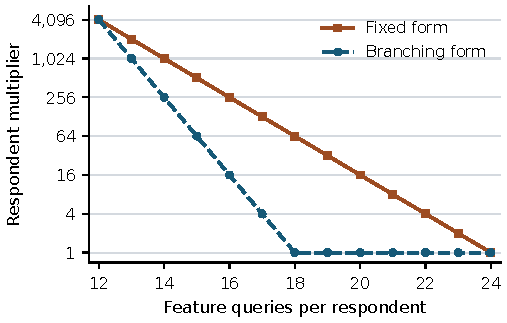
\includegraphics[width=.62\textwidth]{figures/query_cost.pdf}
\caption{Exact synthetic budget curve for the same update on 24 features ($k=6$). The fixed coefficient is 64 and the branching coefficient is one at 18 queries.}
\label{fig:cost}
\end{figure}

\section{Empirical Oracle and Evaluation Details}\label{app:emp}
\subsection{Finite-Sample Oracle for Sequential Designs}
The fixed-form oracle is a pointwise benchmark. Let $z=(x,y)$, $t(z)=yd(x)$, and let $P$ now denote the held-out empirical law. The oracle may use $P$ to select a design and tables, but the resulting estimator must remain unbiased under every possible law. Otherwise the optimization would trivially return the constant $\Delta(P)$. The admissible score functions $H_\iota(\ell_\iota(x),y)$ therefore satisfy
\begin{equation}
             \sum_\iota q_\iota H_\iota(\ell_\iota(x),y)=yd(x)\qquad\text{for every }(x,y).\label{eq:unbpoint}
\end{equation}
Taking the sample mean gives variance $\{\sum_\iota q_\iota\E_P H_\iota^2-\Delta(P)^2\}/n$. The optimum of this one-person score problem is also the exact pointwise optimum over all globally unbiased procedures, including those that choose a later person's form using earlier observations. We state the result for arbitrary finite observation maps to make its scope precise.

\begin{proposition}[Pointwise oracle under sequential form choice]\label{prop:pointwise}
Let $Z$ have an arbitrary law $P$ on a finite space, let $t(Z)$ be known, and let $o_\iota(Z)$ be a finite menu of observation maps whose cells span $t$. Put $\Delta(P)=\E_P t$ and
\begin{equation}
 W(P)=\inf_{q,H:\,\sum_\iota q_\iota H_\iota(o_\iota(z))=t(z)\ \forall z}
       \left\{\sum_\iota q_\iota\E_P H_\iota(o_\iota(Z))^2-\Delta(P)^2\right\}.
 \label{eq:pointwiseoracle}
\end{equation}
Given $n$ iid records, consider protocols that choose the map for person $i$ before observing any part of $Z_i$, using all previous observations and independent randomness. Among estimators that are unbiased under every law and have finite second moment under every law,
\[
       \inf_{\text{such protocols and estimators}}\Var_P(\widehat\Delta)
          =W(P)/n
\]
for every $P$, including laws with zero-mass cells. An iid form mixture and its score mean attain the infimum whenever the program has a minimizer, and otherwise approach it.
\end{proposition}

\begin{proof}
The upper bound follows by using any feasible pair $(q,H)$ independently on the $n$ people. For the converse, first suppose $P$ has full support. For a fixed form law $q$, let $W_q(P)$ be the value in \eqref{eq:pointwiseoracle} with $q$ fixed. Write $c=t-\Delta(P)$ and let $\Pi_\iota h=\E_P[h(Z)\mid o_\iota(Z)]$ on the mean-zero space $L^2_0(P)$. A minimum-norm decomposition gives
\begin{equation}
 W_q(P)=\sup_{h\in L^2_0(P)}
   \frac{\langle c,h\rangle_P^2}{\sum_\iota q_\iota\|\Pi_\iota h\|_{2,P}^2}.
 \label{eq:pointwisedual}
\end{equation}
The value is infinite when the numerator is nonzero and the denominator is zero; $0/0$ contributes zero. To verify the identity, center any feasible score by setting $K_\iota=H_\iota-\Delta(P)$. Its weighted means sum to zero. Subtracting the individual means $\E_P K_\iota$ from the $K_\iota$ preserves $\sum_\iota q_\iota K_\iota=c$ and decreases the objective by $\sum_\iota q_\iota(\E_P K_\iota)^2$. It therefore suffices to minimize $\sum_\iota q_\iota\|K_\iota\|_2^2$ over centered tables with weighted sum $c$. On the product of these centered transcript spaces, the map $K\mapsto\sum_\iota q_\iota K_\iota$ has adjoint $h\mapsto(\Pi_\iota h)_\iota$ in the weighted inner product. Minimum-norm duality, followed by optimization over the scale of $h$, gives \eqref{eq:pointwisedual}. Forms of mass zero are omitted. If the constraint is infeasible, separation gives a zero-denominator witness, so the extended-value identity remains valid.

Fix any admissible sequential protocol and reveal its independent random seed. For a centered $h$, use the submodel $P_\theta(z)=P(z)(1+\theta h(z))$ for sufficiently small $|\theta|$. If person $i$ receives form $A_i$, the likelihood score contributed by that person's observation at $\theta=0$ is $\Pi_{A_i}h(Z_i)$. Form-choice probabilities add no likelihood term because the protocol, conditional on its past observations and seed, is fixed rather than a function of the unknown $\theta$. These scores are martingale differences: $Z_i$ is independent of the previous records and $\E_Ph=0$. Thus the score $S_h$ of the entire experiment satisfies
\begin{equation}
 \E_P S_h^2=n\sum_\iota\bar q_\iota\|\Pi_\iota h\|_{2,P}^2,
 \qquad
 \bar q_\iota=\frac1n\sum_{i=1}^n\Pr_P(A_i=\iota).
 \label{eq:sequentialinformation}
\end{equation}
The probabilities in $\bar q$ may depend on $P$, but $\bar q$ is a valid design distribution for the pointwise oracle. Differentiating global unbiasedness along the submodel gives
\[
 \E_P[(\widehat\Delta-\Delta(P))S_h]=\E_P[ch].
\]
Cauchy--Schwarz and \eqref{eq:pointwisedual} then imply
\[
 \Var_P(\widehat\Delta)\ge W_{\bar q}(P)/n\ge W(P)/n.
\]
This argument allows a nonlinear estimator and arbitrary dependence of later forms on earlier observations.

It remains to treat a law $P$ on the boundary of the simplex. Let $P_\epsilon=(1-\epsilon)P+\epsilon P_0$ for a fixed full-support law $P_0$. For a fixed protocol, condition on the entire sequence of latent full records and average only over its independent random seed. Since the record space is finite and the estimator has finite second moment under $P_0$, every resulting conditional second moment is finite. The estimator's first and second moments are therefore finite polynomials in the cell probabilities; in particular its variance is continuous at $P$. If $F(P)=W(P)+\Delta(P)^2$, the feasible set defining $F$ is population-independent and its objective is linear in the population law for each design. Hence
\[
 F(P_\epsilon)\ge(1-\epsilon)F(P),\qquad
 \liminf_{\epsilon\downarrow0}W(P_\epsilon)\ge W(P).
\]
Apply the already proved lower bound at $P_\epsilon$ and pass to the limit. This proves the result at every law.
\end{proof}

For our empirical benchmark, take $Z=(X,Y)$, $t(Z)=Yd(X)$ and $o_T(Z)=(X_T,Y)$. Each fixed form must be chosen before the current person's features or label are seen, as in Section~2. The proposition applies conditionally on the frozen training data. Its oracle chooses a protocol using $P$, then requires that same protocol and estimator to be unbiased under every alternative law. This permits a distribution-specific benchmark without allowing the trivial constant estimator $\Delta(P)$. The lower bound covers predetermined form counts and adaptation across respondents. It does not cover estimators that are biased at other populations, such as the fitted imputation comparator.

\subsection{Computing and Evaluating the Oracle}
All three-feature-and-label marginals used in the numerical solvers were positive, although the proposition also permits empty full-profile cells.


\section{Learning a Design from a Compact Tree}\label{app:pathdesign}
Fix a tree that recovers $t(z)=yd(x)$ within $b$ distinct queries. Pad each path deterministically to $b$ coordinates. Enumerate its distinct path sets $\mathcal S=\{S_1,\ldots,S_L\}$ and let $S(z)$ denote the reached set. If an assigned fixed form $S_j$ permits following the padded tree to completion, then $S(z)=S_j$, as in Appendix~\ref{app:universal}. For any strictly positive form law $q$, the score
\[
 H_q(z,J)=\frac{t(z)}{q_J}\mathbf1\{S(z)=S_J\},\qquad J\sim q,
\]
is computable from the selected form and label. It is unbiased conditional on every full record. With $w_j=\E_P[t(Z)^2\mathbf1\{S(Z)=S_j\}]$,
\begin{equation}
 \Var_P H_q=\sum_{j=1}^L\frac{w_j}{q_j}-\Delta(P)^2.
 \label{eq:pathvariance}
\end{equation}
Within this importance-score family the unconstrained optimum is $q_j\propto\sqrt{w_j}$, with infimal second moment $(\sum_j\sqrt{w_j})^2$. Zero-mass cells are handled by limits. We enforce $q_j\ge\beta/L$ with $\beta=0.1$, ensuring global unbiasedness even on path sets absent from calibration. If some $w_j>0$, the constrained optimum satisfies $q_j=\max\{\beta/L,c\sqrt{w_j}\}$, with $c$ chosen to normalize the probabilities. If all weights vanish, every feasible $q$ is optimal. Iteratively fixing cells below the floor computes the positive-weight solution without profile enumeration. This oracle optimizes a specified score family, not all fixed-form estimators.

\subsection{A Worked Two-Question Example}
Let $d(x)=[(1+x_1)x_2+(1-x_1)x_3]/2$. Branching queries $x_1$ and then $x_2$ when $x_1=1$, or $x_3$ when $x_1=-1$. The two fixed forms are
\begin{center}
\begin{tabular}{lll}
\toprule
Form & Probability & Observed score\\
\midrule
$\{1,2\}$ & $1/2$ & $2Yx_2\mathbf1\{x_1=1\}$\\
$\{1,3\}$ & $1/2$ & $2Yx_3\mathbf1\{x_1=-1\}$\\
\bottomrule
\end{tabular}
\end{center}
At every full record the mean score is $Yd$ and its second moment is two. The branching score has second moment one. For an independent fair label both score means vanish, so their sample-mean variances are exactly $2/n$ and $1/n$. This describes these concrete estimators; the minimax results additionally justify their worst-case comparison against all protocols.

\subsection{A Finite Calibration Guarantee}
Suppose the tree is fitted independently of $r$ calibration records and $|t|\le M$. Full calibration records reveal $W_j=t^2\mathbf1\{S=S_j\}$ directly. Alternatively, assign each calibration person a uniformly random fixed path set. On successful completion return $W_j=L t^2\mathbf1\{J=j,S=S_j\}$ and return zero on failure. This alternative obeys the same fixed per-person cap and uses only observable quantities. In both cases $\E W=w$. Let $\widehat w$ be the mean and let $\widehat q$ minimize $\sum_j\widehat w_j/q_j$ subject to $q_j\ge\beta/L$.

\begin{proposition}[Learning path-set probabilities]\label{prop:pilot}
Let $q_\beta^\star$ be the population optimum with the same probability floor. Set $B=M^2$ for full calibration or $B=LM^2$ for uniformly assigned fixed calibration. With probability at least $1-\alpha$ over the $r$ independent calibration records,
\[
 \Var_P H_{\widehat q}-\Var_P H_{q_\beta^\star}
 \le\frac{2LB}{\beta}\sqrt{\frac{2(L\log2+\log(1/\alpha))}{r}}.
\]
The resulting audit mean on fresh respondents remains globally unbiased for every realized calibration sample.
\end{proposition}
\begin{proof}
Each calibration vector has at most one nonzero entry and $\|W\|_1\le B$. For any sign vector $\sigma\in\{-1,1\}^L$, $\sigma^TW\in[-B,B]$. Hoeffding's inequality and a union bound over $2^L$ vectors give
\[
 \|\widehat w-w\|_1
 =\max_\sigma\sigma^T(\widehat w-w)
 \le B\sqrt{2(L\log2+\log(1/\alpha))/r}.
\]
The difference between the empirical and population second-moment objective is uniformly at most $(L/\beta)\|\widehat w-w\|_1$. Empirical minimization costs at most twice this uniform deviation. Subtracting the common $\Delta^2$ proves the bound. Pointwise conditional unbiasedness holds for each positive $q$, hence also conditional on the entire calibration sample.
\end{proof}
The bound is conservative and becomes informative only with sufficiently large calibration samples. It proves consistency relative to a constrained family oracle, not a calibration-free optimality claim. Form enumeration takes time polynomial in the given tree's size and $m$; that tree may itself have exponentially many leaves in $b$. A deployment needs only its form probabilities and the tree, not a table over all $s^m$ profiles.

\subsection{Higher-Dimensional Benchmark}
SUSHI uses all 28 pairwise comparisons among the eight items outside each target pair. SAPA uses the first twenty other items in the fixed order A1--A5, C1--C5, E1--E5, N1--N5, O1--O5, dropping rows missing any selected item or target. A separate SAPA-ordinal condition retains the original six-valued features; its target is still binary at threshold four. Feature choices use neither labels nor held-out performance. SUSHI pairwise features are dependent, and no independence assumption is used to evaluate risk.

The current main experiment uses one fixed person-level permutation, seed 20261106. The first 800 complete records fit a depth-six CART tree with minimum leaf size 25; the next 500 calibrate the score; the remainder define the empirical population. The old rule uses the root child's frequency and the new rule the reached leaf frequency. This is a controlled refinement, chosen because the target is exactly computable by branching within the cap. Both binary datasets' full target lists are included. Ordinal and depth-three results remain secondary diagnostics in Appendix~\ref{app:operational}.

Calibration-only fitting and the empirical-population oracle use the same frozen rules and evaluation population. The supplied path menu is a tractable implementation choice. All-form lower bounds in the supplementary report separately certify the loss beyond that menu.

\subsection{Confidence Intervals and Costs}
Conditional on calibration, each path score has magnitude at most $M/q_{\min}$. Thus the ordinary score mean has a distribution-free $(1-\alpha)$ confidence interval with half-width
\[
 \frac{M}{q_{\min}}\sqrt{\frac{2\log(2/\alpha)}n},
\]
intersected with $[-M,M]$. The branching score has the same bound with $q_{\min}=1$. These Hoeffding intervals are valid but conservative; they are not claims of optimal interval width or power. The paper's risk comparisons concern MSE and do not order intervals for biased estimators.

For a menu with known per-person costs $c_\iota>0$, let $c(q)=\sum_\iota q_\iota c_\iota$. An iid unbiased score mean with $n$ respondents uses expected cost $nc(q)$, so its worst-case MSE-times-cost upper criterion is $c(q)\max_x\sum_\iota g_\iota(x)^2/q_\iota$. Set $r_\iota=q_\iota/c(q)$. Joint cost-weighted design becomes the convex program
\[
 U_c(d,\A)=\inf_{\substack{r,g:\,\sum_\iota c_\iota r_\iota=1\\ \sum_\iota g_\iota=d}}
              \max_x\sum_\iota\frac{g_\iota(x)^2}{r_\iota}.
\]
Conversely $q_\iota=r_\iota/\sum_jr_j$ recovers the design, proving equivalence of the two criteria. For fixed forms, $c_\iota$ may include recruitment, the label and item-specific costs. For a branching tree, taking $c_\iota$ as its maximum path cost gives a conservative criterion. This uses expected total expenditure and continuous sample-size scaling; it does not impose an almost-sure stopping budget or establish a sharp adaptivity ratio for arbitrary costs.



\section{Instance Certificates, Rounds and Observation Timing}\label{app:instances}
\subsection{Instance-Specific Coefficients}
Suppose a depth-$b$ tree $\tau$ computes $d$ exactly, let $M=\|d\|_\infty>0$, and let $L_\tau$ be its number of distinct padded path sets. Under the uniform law on the binary cube, put
\[
 E_b(d)=\max_{|T|\le b}\sum_{S\subseteq T}\widehat d(S)^2.
\]
Then
\begin{equation}
 \max\left\{1,\frac{\|d\|_{2,\U}^4}{M^2 E_b(d)}\right\}
 \le \frac{V_{\rm fixed}(d,b)}{V_{\rm branch}(d,b)}
 \le \min\{L_\tau,K_{m,b}\},\qquad V_{\rm branch}(d,b)=M^2.
 \label{eq:instanceinterval}
\end{equation}
Indeed the tree score $d$ has maximum second moment $M^2$, while Jensen gives that lower bound for every unbiased representation. The variance dual with $\mu=\U,h=d$ gives the first inequality; Parseval identifies its denominator as $E_b(d)$. Simulating $\tau$ gives the $L_\tau$ bound, and the universal theorem supplies $K_{m,b}$. This certificate is instance-specific but still concerns worst-case populations. It does not bound the ratio $W(P)/\Var_P(Yd)$ at an individual population by the same instance coefficient ratio: the denominator of that latter ratio is a population variance, not $M^2$.

The path-set bound need not be attainable for a given tree. On four
coordinates with cap three, take the chain querying $X_4$, stopping on its
negative branch, then querying $X_3$, stopping on its negative branch,
and otherwise querying $X_2$. Padding early leaves with the smallest unused
coordinates yields the three sets $\{1,2,4\}$, $\{1,3,4\}$ and
$\{2,3,4\}$, so $L_\tau=3$. Nevertheless every assignment of values to
the original leaves depends only on $X_2,X_3,X_4$. One fixed triple
computes it, and the coefficient ratio is one for every nonzero assignment.
Thus $L_\tau$ is a simulation upper bound and can depend on padding; it
is not a sharp invariant of every underlying tree.

For four features, our coefficient solver minimizes $v$ subject to $\sum_\iota M_\iota g_\iota=d$, $\sum_\iota q_\iota=1$, and $\sum_\iota g_\iota(x)^2/q_\iota\le v$ on all sixteen profiles. Here $M_\iota$ lifts a triple-score table. An implementable score supplies an upper bound. A nonnegative probability vector $\mu$ and arbitrary vector $h$ supply the lower bound
\[
 \frac{(h^Td)^2}{\max_\iota\sum_C (\sum_{x\in C}h_x)^2/\mu(C)},
\]
where $C$ ranges over form $\iota$'s cells. This follows directly from Cauchy--Schwarz applied to every unbiased decomposition. We normalize the nonnegative state dual, add $10^{-12}$ mass per state, and evaluate this expression; no solver-reported objective is treated as a certificate without reconstruction. The returned primal tables are projected onto the exact observation-span constraint. The supplement records both bounds and the numerical equality residual.

\subsection{An Exact Four-Feature Example Beyond the Block Gap}\label{app:fourbit}
The ratio two in the four-bit block is not extremal at $(m,b)=(4,3)$.
\begin{proposition}\label{prop:fourbit}
There is a Boolean contrast on four features, computable by a depth-three tree, with
\[
 V_{\rm branch}(d,3)=1,\qquad
 V_{\rm fixed}(d,3)=\frac{7+2\sqrt2}{4}=2.457106\ldots.
\]
\end{proposition}
\begin{proof}
Write $\zeta=\sqrt2$ and $\alpha=(7+2\zeta)/4$. Define
\[
 f_-(x)=\frac{(1-x_2)x_1-(1+x_2)x_3}{2},\qquad
 f_+(x)=-\frac{(1-x_3)x_2+(1+x_3)x_1}{2},
\]
\[
 d(x)=\frac{(1-x_4)f_-(x)+(1+x_4)f_+(x)}2.
\]
Query $x_4$ first. If its value is $-1$, query $x_2$ and then $x_1$ or $x_3$; if its value is $+1$, query $x_3$ and then $x_2$ or $x_1$. This computes $d\in\{-1,1\}$ with three queries. Jensen's inequality and the exact tree score give $V_{\rm branch}=1$.

For the fixed upper bound use only the forms $124$, $134$ and $234$, with respective probabilities $(2-\zeta)/2$, $(2-\zeta)/2$ and $\zeta-1$. In a form $T=(i,j,k)$ index its answers by $c=(1+x_i)/2+2(1+x_j)/2+4(1+x_k)/2$. The following table specifies twice the unbiased decomposition table $g_T$; the returned score is $Yg_T/q_T$.
\begin{center}
\begin{tabular}{rrrr}
\toprule
$c$ & $2g_{124}$ & $2g_{134}$ & $2g_{234}$\\
\midrule
0 & $\zeta-3$ & $4-3\zeta$ & $2\zeta-3$\\
1 & $3-\zeta$ & $2-\zeta$ & $2\zeta-1$\\
2 & $\zeta-1$ & $\zeta-2$ & $3-2\zeta$\\
3 & $1-\zeta$ & $3\zeta-4$ & $1-2\zeta$\\
4 & $2-\zeta$ & $1-\zeta$ & $2\zeta-1$\\
5 & $4-3\zeta$ & $\zeta-1$ & $1-2\zeta$\\
6 & $3\zeta-4$ & $3-\zeta$ & $2\zeta-3$\\
7 & $\zeta-2$ & $\zeta-3$ & $3-2\zeta$\\
\bottomrule
\end{tabular}
\end{center}
Number full profiles lexicographically by $i=8(1+x_1)/2+4(1+x_2)/2+2(1+x_3)/2+(1+x_4)/2$, and put $E=\{1,2,3,6,8,12,13,15\}$. Substitution gives $\sum_Tg_T=d$ on all sixteen profiles. The conditional second moment equals $\alpha$ on $E$, and $(23-10\zeta)/4$ outside $E$. The latter is smaller because their difference is $3\zeta-4>0$. Thus $V_{\rm fixed}\le\alpha$.

For the matching lower bound, let $\mu$ be uniform on $E$. Set $\xi=3+2\zeta$ and define a signed vector $\eta$, in the same full-profile order, by
\[
 32\eta=(-\xi,3,-5,5,\xi,-\xi,-3,\xi,5,\xi,\xi,-\xi,3,-3,-\xi,-5).
\]
For a form $T$ let $I_T=\sum_C\eta(C)^2/\mu(C)$ over its cells, with $0/0=0$. Every zero-mass cell in this example also has zero signed mass. Direct summation yields
\[
 \eta^Td=\alpha,\qquad
 I_{123}=\alpha-\frac12,\qquad
 I_{124}=I_{134}=I_{234}=\alpha.
\]
The Cauchy--Schwarz certificate above therefore gives $V_{\rm fixed}\ge(\eta^Td)^2/\max_T I_T=\alpha$. Forms with fewer coordinates are coarsenings of triples and cannot increase $I_T$. All displayed identities are exact in $\mathbb Q(\sqrt2)$; the supplied symbolic script verifies them without a numerical optimizer.
\end{proof}
Consequently the worst ratio at $(4,3)$ lies in $[(7+2\sqrt2)/4,3]$. This excludes two as its value, but neither proves that three is attainable nor determines the exact supremum over all identifiable real contrasts.

\begin{corollary}\label{cor:roundseparation}
For the same contrast and budget three, $V_2(d,3)\ge4/3>V_{\rm branch}(d,3)=1$.
\end{corollary}
\begin{proof}
Use the uniform law and witness $h=d$. A deterministic two-round protocol can be represented by a first set $S$ of size one or two, followed by a set of $3-|S|$ remaining coordinates depending on the first answers. Padding covers protocols using fewer queries; a single fixed triple is included by splitting it into a first pair and a final fixed coordinate. For a given $S$, its largest possible projection energy is
\[
 J(S)=2^{-|S|}\sum_{u\in\{-1,1\}^S}
 \max_{\substack{T\subseteq[4]\setminus S\\|T|=3-|S|}}
 \E\!\left[\E[d\mid X_S=u,X_T]^2\mid X_S=u\right].
\]
Substitution of the displayed contrast gives the complete table:
\begin{center}
\begin{tabular}{ll}
\toprule
First set $S$ & $J(S)$\\
\midrule
$\{1\},\{4\},\{1,2\},\{1,3\},\{1,4\},\{2,3\}$ & $1/2$\\
$\{2\},\{3\},\{2,4\},\{3,4\}$ & $3/4$\\
\bottomrule
\end{tabular}
\end{center}
Thus every allowed two-round observation has projection energy at most $3/4$. The variance dual with $\E[d^2]=1$ gives $V_2\ge4/3$, including mixtures of these protocols. The symbolic script also verifies all ten entries using rational arithmetic. This is a strict constant separation; an exponential two-round-versus-full separation is not established here.
\end{proof}


\subsection{Two Rounds Already Attain the Universal Extremum}\label{app:rounds}
An $R$-round interview uses at most $R$ batches, choosing each batch of coordinates using only the preceding batches' answers, with at most $b$ coordinates in total. Let $V_R$ use all such interviews. One round is the fixed-form menu and $b$ rounds suffice for full branching. For any $R\ge2$,
\[
 1\le V_{\rm fixed}/V_R\le K_{m,b},\qquad
 \sup_{m,d\ne0}\frac{V_{\rm fixed}(d,b)}{V_R(d,b)}=2^{b-1},
\]
where the supremum is over identifiable binary contrasts. The upper bound follows from menu inclusion. The address construction attains equality using two batches: all address bits, then the addressed data bit. Thus the universal extremum measures the value of permitting a second batch; it does not require $b$ sequential rounds.

The block construction also needs at most two rounds throughout its identifiable budget curve. At $b=2k+R$, $0\le R\le k$, use the paper's three-query strategy on $R$ blocks and two-query strategy on the others. Ask the first two queries in every block together; then ask the selected third coordinate in the $R$ adaptive blocks. At $b\ge3k$ this already evaluates the contrast exactly. The address and block examples do not separate two rounds from unrestricted branching. Corollary~\ref{cor:roundseparation} supplies such a constant separation with a different four-feature contrast; a general exponential hierarchy remains unsettled here.

\subsection{Labels and Across-Person Adaptation}
Let $R_{\rm pre}$ require selecting the interview independently of the current label, and let $R_{\rm label}$ allow observing that label first, while both permit adaptation across people. For an identifiable contrast, Theorem~\ref{thm:asym} and the iid upper construction imply
\[
 \lim_{n\to\infty}nR_{\rm pre}(d,n)
 =\lim_{n\to\infty}nR_{\rm label}(d,n)=V(d,\A).
\]
Thus neither access to earlier people nor early access to the current label reduces the first-order worst-case coefficient relative to an optimal iid design.

There is also an exact statement for the \emph{finite program}. If one extends $\Phi_n$ to separate form laws and score tables for $y=-1,+1$, its objective is the maximum over these labels of their individual worst-profile quadratic objectives. Multiplying the negative-label tables by $-1$ turns both subproblems into the definition of $\Phi_n(d,\A)$. Each has value at least $\Phi_n$, and using the same form law and sign-adjusted tables attains it. Early labels therefore do not improve this program. This is not an equality claim for the exact finite-$n$ minimax risks, which the program bounds only within a constant.

\section{Efficiency and Augmented Fixed Forms}\label{app:augmentation}
\subsection{Relation to the Missing-Data Efficiency Bound}
Fix a known form law $q$ and a full-support law $P$ on the finite complete-record space. The observed record is $O=(A,o_A(Z))$. Its score along a centered complete-data perturbation $h$ is $\E_P[h(Z)\mid O]$. A mean-zero observed influence function $\phi(O)$ for $\Delta=\E_Pt$ must therefore satisfy
\[
 \E[\phi(O)\mid Z]=t(Z)-\Delta.
\]
Conversely this equation gives the required pairing with every complete-data score, and hence an influence function in this finite regular model. Minimizing $\E\phi^2$ is the efficiency bound. Substituting $\phi=H-\Delta$ identifies it with the fixed-design population variance $W_q(P)$ (the finite-sample oracle of the supplementary report). This is the usual known-coarsening influence-function geometry \citep{robins1994,tsiatis2006}, not a new asymptotic efficiency formula. The proposition's additional statement is finite-$n$ pointwise optimality over globally unbiased nonlinear estimators and sequential form assignments, together with its extension to boundary laws. It does not assert a finite-sample bound for all locally regular biased estimators.

Fixed random forms implement planned missingness. A tree's terminal cell is generated using observed answers, so its known acquisition mechanism is a designed coarsening-at-random mechanism \citep{heitjan1991,gill1997}. This description does not cover arbitrary unrecorded selection or nonresponse.

\subsection{Common-Feature Augmentation}
All padded path sets contain the root feature. For any fixed function $c=c(X_{\rm root},Y)$ and positive $q$, the observable score
\[
 H=c+\frac{\mathbf1\{S=S_J\}}{q_J}(t-c)
\]
has conditional mean $t$ at every complete record. Its variance is
\[
 \Var H=\Var t+\E[(q_{S}^{-1}-1)(t-c)^2].
\]
Both identities follow by averaging over the independently assigned form. A fitted $c$ need not improve held-out variance. Our root comparator uses the calibration mean in each root-value-and-label cell, with one pseudo-observation at the overall mean, and the original fitted path-form law.

\subsection{Optimizing Scores on Observed Prefixes}\label{app:prefix}
A fixed form can follow the tree until the next requested coordinate is unavailable. Record that stopping node (or the reached leaf) and the label. For a tree with $K$ leaves, each form induces a partition of the $K$ leaves: all leaves below a stopping node belong to one cell. This transcript is computable solely from the assigned form. Let $M_\iota$ be its leaf-to-cell incidence matrix and $d_\ell$ the known contrast at leaf $\ell$. For a calibrated joint law $\widehat p(\ell,y)$, solve
\begin{equation}\label{eq:mainprefix}
 \min_{q,g}\sum_{\iota,y,C}\widehat p_y(C)\frac{g_{\iota,y,C}^2}{q_\iota},
 \qquad \sum_\iota M_\iota g_{\iota,y}=y d,\quad
 \sum_\iota q_\iota=1,\quad q_\iota\ge\beta/L.
\end{equation}
This is a convex quadratic-perspective program with $2K$ equality constraints and at most $2LK$ score entries. It is polynomial in the supplied tree/menu representation and numerical precision under the usual conic-optimization model, without enumerating $s^m$ raw profiles. The output score $g_{\iota,y,C}/q_\iota$ is globally unbiased because the equality holds on every leaf for either label. The optimum is only for this specified prefix transcript and form menu.

The original completion-only score is feasible in this program. So is a root augmentation that is constant on the prefix cells, including the binary-root comparator. At the same reference law the optimum weakly improves these contained score families. With ordinal features, the full root value can distinguish records within a prefix cell; the corresponding root comparator is not necessarily contained in this program. For positive cell masses, eliminating the scores gives an efficient numerical formulation. Set $D_{\iota,y}=\operatorname{diag}(\widehat p_y(C))$ and
\[
 A_y(q)=\sum_\iota q_\iota M_\iota D_{\iota,y}^{-1}M_\iota^T,\qquad
 F(q)=\sum_y d^T A_y(q)^{-1}d.
\]
Every leaf is a singleton in at least one path form, so $A_y(q)$ is positive definite. Its gradient is the negative cell-weighted squared score. The tangent gives a lower certificate over the floored simplex; reconstructed scores give a feasible upper value. Calibration uses one half-count per leaf-and-label state. The model, calibration sample and evaluation sample remain disjoint as in Appendix~\ref{app:pathdesign}. The current primary-split comparisons use the same trees, respondents and caps across score families. Calibration optimality need not imply optimality at the evaluation population.

\section{A Computable Workflow for Dense Updates}\label{app:dense}
On a finite binary cube let $\mathsf F$ contain the $p$ parity columns of degrees at most $b$. Compute the identification floor by the linear program
\[
 \delta=\min_{\gamma\in\mathbb R^p,e\ge0}\{e:-e\mathbf1\le d-\mathsf F\gamma\le e\mathbf1\},
\]
where only $e$ is constrained to be nonnegative and $\gamma$ is unrestricted. A dual witness $h$ with $\mathsf F^Th=0$ and $\|h\|_1\le1$ certifies $\delta\ge h^Td$. For an audit of size $n$, select a variance-aware approximation by minimizing
\[
 \|d-\mathsf F\gamma\|_\infty^2+\|\gamma\|_1^2/n.
\]
For each respondent draw a parity term $S$ with probability $|\gamma_S|/\|\gamma\|_1$, ask its at most $b$ coordinates, and return $Y\operatorname{sgn}(\gamma_S)\|\gamma\|_1\chi_S(X)$. The empty term requires no feature. If all coefficients vanish, return zero. The conditional mean is $Y(\mathsf F\gamma)(X)$ and the second moment is $\|\gamma\|_1^2$, proving the displayed uniform MSE bound. This converts approximation into an implementable audit while reporting the unavoidable lower floor $\delta^2$ separately.

The demonstration uses the primary split of all 45 SUSHI and 25 binary SAPA targets, taking the first eight of the larger benchmark's features. Logistic regressions fitted on 800 records use respectively the first four and all eight features; their predicted positive-class probabilities define the old and new rules. Regularization is $C=1$ with a 1,000-iteration cap. On all $2^8$ profiles we compute the degree-three linear program and the variance-aware approximation for $n=1000$, then evaluate its exact score moments on the remaining respondents. The floor treats all 256 binary profiles as admissible; a smaller support reflecting ranking consistency defines a different identification problem. This is an executable eight-feature workflow; full-cube enumeration remains exponential in dimension. In larger problems it requires a certified optimization or approximation oracle, not just evaluation on a calibration sample.



\section{Products of Addresses and Equality Certificates}\label{app:structure}
\subsection{Nearly Maximal Gaps in Polynomial Dimension}\label{app:productaddress}
For $\kappa\ge0$, an address block consists of $\kappa$ address bits and $2^\kappa$ data bits, and returns the addressed data bit. At $\kappa=0$ it is just one data bit. Let $f_j$ be address blocks on disjoint coordinates, with address lengths $\kappa_1,\ldots,\kappa_k$, and put
\[
 d=\prod_{j=1}^k f_j,\qquad
 b=\sum_{j=1}^k(\kappa_j+1),\qquad
 m=\sum_{j=1}^k(\kappa_j+2^{\kappa_j}),\qquad D=2^{\sum_j \kappa_j}.
\]
\begin{proposition}[Product address coefficient]\label{prop:productaddress}
For this contrast, $V_{\rm branch}(d,b)=1$ and $V_{\rm fixed}(d,b)=D=2^{b-k}$. Two rounds attain the branching coefficient.
\end{proposition}
\begin{proof}
Query all address bits first, and the $k$ selected data bits second. This evaluates $d$ within budget $b$, giving coefficient one by Jensen's inequality. For a fixed design, independently guess one data index in each block, query those $k$ bits and all address bits, and return $D d$ if every guess matches, zero otherwise. Completion has probability $1/D$ at every profile, so the conditional mean is $d$ and second moment is $D$.

For the converse let $\mu$ be uniform on the full cube and use $h=d$ in the variance dual. An arbitrary fixed form can allocate its queries among blocks in any way. If it observes $s_j$ address bits and $r_j$ data bits in block $j$, independence gives
\[
 \|\E_\mu[d\mid X_T]\|_2^2
 =\prod_{j=1}^k r_j2^{s_j-2\kappa_j}.
\]
If some $r_j=0$, this is zero. Otherwise $r_j\le2^{r_j-1}$ and $\sum_j(s_j+r_j)\le b$, whence
\[
 \prod_j r_j2^{s_j-2\kappa_j}
 \le 2^{\sum_j(s_j+r_j)-k-2\sum_j \kappa_j}
 \le 2^{-\sum_j \kappa_j}=D^{-1}.
\]
Since $\E_\mu[dh]=1$, the variance dual gives $V_{\rm fixed}\ge D$. This treats all fixed forms, including those that redistribute queries across blocks. The general minimax theorem then covers arbitrary biased estimators and history-dependent form selection.
\end{proof}

For any fixed $\kappa\ge1$, equal blocks give
\[
 m=\frac{\kappa+2^\kappa}{\kappa+1}b,\qquad
 \frac{V_{\rm fixed}}{V_{\rm branch}}=2^{\kappa b/(\kappa+1)}
 \quad\text{when }\kappa+1\text{ divides }b.
\]
In particular $m=3b/2$ permits $2^{b/2}$. More generally, for any fixed $\zeta>0$ one can choose a constant $\kappa$ so that the exponent is at least $(1-\zeta)b$ while $m=O_\zeta(b)$; the hidden dimension multiplier grows with $1/\zeta$. This does not solve the sharp frontier for a prescribed ratio $m/b$, such as $4/3$.

For every $b\ge2$, choose $\kappa=\lfloor\log_2 b\rfloor$, $k_0=\lfloor b/(\kappa+1)\rfloor$, and $\rho_0=b-k_0(\kappa+1)$. Use $k_0$ blocks of address length $\kappa$ and $\rho_0$ blocks of address length zero. Then $m=k_0(\kappa+2^\kappa)+\rho_0\le b^2$, and
\[
 \log_2(V_{\rm fixed}/V_{\rm branch})
 =k_0\kappa=b-k_0-\rho_0
 \ge b-\frac{b}{\kappa+1}-\kappa.
\]
Thus polynomial dimension already permits $2^{b-O(b/\log b)}$. The construction uses the standard product method; the content is the exact coefficient and the lower bound uniform over all query allocations.

\subsection{When the Full-Information Coefficient Is Attained}\label{app:equality}
Write $M=\|d\|_\infty>0$ and let $\mathcal H_\iota$ be the space of functions observable under interview $\iota$. Define the bounded-decomposition quantity
\[
 \mathcal C_\A(d)=\inf\left\{\sum_\iota\|g_\iota\|_\infty:
       g_\iota\in\mathcal H_\iota,\ \sum_\iota g_\iota=d\right\}.
\]
It is computed by a linear program: minimize $\sum_\iota u_\iota$ subject to $\sum_\iota g_\iota=d$ and $-u_\iota\le g_\iota(c)\le u_\iota$ on every cell. Its size is that of the enumerated profiles and menu, not polynomial in a general compact representation.

\begin{proposition}[Equality and a bounded-score certificate]\label{prop:equality}
For any identifiable $d$, $M\le \mathcal C_\A(d)$ and
\[
 M^2\le V(d,\A)\le \mathcal C_\A(d)^2.
\]
Consequently $\mathcal C_\A(d)=M$ suffices for $V(d,\A)=M^2$. Equivalently, it suffices that $d/M$ be a convex combination of observable functions with values in $[-1,1]$.
If $|d(x)|=M$ at every profile, then $V(d,\A)=M^2$ if and only if one interview in $\A$ computes $d$ exactly. In particular, a Boolean contrast on the full cube has $V_{\rm fixed}(d,b)=1$ if and only if it depends on at most $b$ coordinates.
\end{proposition}
\begin{proof}
The triangle inequality gives $\mathcal C_\A(d)\ge M$. For a decomposition of total norm $C$, choose $q_\iota=\|g_\iota\|_\infty/C$, dropping zero terms. Each returned score $g_\iota/q_\iota$ is bounded by $C$, giving $V\le C^2$. Jensen gives $V\ge M^2$.

For the last assertion the finite program attains its optimum: a bounded objective bounds every $g_\iota$, the simplex is compact, and the quadratic perspectives are closed at $q_\iota=0$. At an optimum with value $M^2$, for each profile,
\[
 d(x)^2=\left(\sum_\iota q_\iota H_\iota(x)\right)^2
 \le\sum_\iota q_\iota H_\iota(x)^2\le M^2.
\]
If $|d(x)|=M$ everywhere, equality in Jensen forces $H_\iota(x)=d(x)$ for every positive-weight interview and every profile. Any such interview computes $d$. The converse follows by using that interview alone. A fixed coordinate set computes $d$ precisely when it contains all of its relevant coordinates.
\end{proof}

For general real-valued $d$, equality in Jensen is forced only on the extremal set $E=\{x:|d(x)|=M\}$. Every used form must distinguish opposite-sign extremal profiles. That condition is necessary but does not by itself control second moments away from $E$. The bounded-decomposition test is a sufficient certificate; it is not asserted to be necessary for general $d$. Deterministic classifier differences take values in $\{-1,0,1\}$, so they are not covered by the constant-magnitude equivalence when zero contrasts occur.

Few extremal profiles alone do not imply a small gap. Take an even number $k\ge2$ of equal address blocks of length $\kappa\ge1$, let $f$ be their product, and put $\ell(x)=m^{-1}\sum_{i=1}^m x_i$. For $0<\epsilon<1$ define $d_\epsilon=(1-\epsilon)f+\epsilon\ell$. The only profile with $|d_\epsilon|=1$ is the all-positive profile: $\ell=\pm1$ only at the two constant profiles, and $f=1$ at both when $k$ is even. A mixture of the two-round exact score for $f$ and a uniformly sampled one-coordinate score for $\ell$ has magnitude one and conditional mean $d_\epsilon$, so $V_{\rm branch}=1$. Under the uniform law, $\E[f\ell]=0$ because any coordinate lies in only one block and another independent block has zero mean. The witness $h=f$ from Proposition~\ref{prop:productaddress} therefore gives
\[
 V_{\rm fixed}(d_\epsilon,b)\ge(1-\epsilon)^2 2^{k\kappa}.
\]
An exponentially large gap is therefore compatible with a non-Boolean contrast having a unique absolute maximum. Empirical near-equality should be established by certificates rather than inferred from extremal-profile counts.

\subsection{Optimizing a Root Augmentation}\label{app:weightedroot}
With $U=(X_{\rm root},Y)$ and $w=q_S^{-1}-1$, the variance identity in Appendix~\ref{app:augmentation} implies that, for fixed $q$, the population-optimal root function is
\[
 c^*(U)=\frac{\E[wt\mid U]}{\E[w\mid U]},
\]
with any value when the denominator is zero. This follows by minimizing the conditional quadratic $\E[w(t-c)^2\mid U]$. The weighted calibration counterpart uses the same form law as the original comparator and a single pseudo-observation at the calibration grand mean, weighted by the mean calibration weight. It remains globally unbiased. A reduction in its calibration criterion does not guarantee a reduction under the held-out law.

\subsection{One-Sided Deterministic Updates Can Have an Exponential Gap}
\label{app:indicatoraddress}
Large global gaps do not require complementary classifiers. Let $A$ have
$\kappa\ge1$ address bits, let $D=2^\kappa$, and write $Z_j\in\{0,1\}$
for its data bits. The old rule always predicts $-1$, and the new rule
predicts $+1$ exactly when $Z_A=1$. Their contrast is $d=Z_A\in\{0,1\}$.
\begin{proposition}\label{prop:indicatoraddress}
For this contrast, $m=\kappa+D$, $b=\kappa+1$, and
\[
 V_{\rm branch}(d,b)=1,\qquad
 V_{\rm fixed}(d,b)=\frac{D^2}{4(D-1)}.
\]
The ratio is asymptotic to $2^{b-3}$. Multiplying the contrast by any
$\epsilon\in(0,1]$ leaves the ratio unchanged.
\end{proposition}
\begin{proof}
Put $\pi=D/[2(D-1)]$. Choose a data index $J$ uniformly, query all address
bits and $Z_J$, and return the feature score
\[
 H=\pi+D\mathbf1\{J=A\}(Z_J-\pi).
\]
Its conditional mean is $d$. If $J=A$, its value is $D(d-1/2)$; otherwise
it is $\pi$. Hence its conditional second moment is
$D/4+(D-1)\pi^2/D=D^2/[4(D-1)]$ for either value of $d$.

For the converse, let $\mu$ have a uniform address and independent
Bernoulli$(\pi)$ data bits, and take $h=\pi+D(d-\pi)$.
A fixed form with $s$ address bits and $r$ data bits has
\[
 \|\E_\mu[h\mid X_T]\|_\mu^2
 =\pi^2+\pi(1-\pi)r2^s
 \le\pi^2+D\pi(1-\pi)=:F,
\]
because $r+s\le\kappa+1$ implies $r2^s\le D$.
Also $\langle d,h\rangle_\mu=D\pi-(D-1)\pi^2=F$.
The variance dual therefore gives $V_{\rm fixed}\ge F=D^2/[4(D-1)]$.
This calculation includes $D=2$, where $\pi=1$ and the lower bound is
simply one. Branching evaluates $d$ exactly, and Jensen gives its matching
coefficient one. Both coefficients scale by $\epsilon^2$.
\end{proof}

This is a constructed model family, not a claim about how frequently
trained classifiers have such gaps. It separates the structural question
from model-family labels: a GBDT or neural-network name alone determines
neither identifiability nor the global efficiency ratio.


\section{Expected Budgets and a Local Efficiency Comparison}\label{app:costlocal}
\subsection{The Expected-Budget and Hybrid Address Coefficients}\label{app:expectedproof}
A mean feature budget $b$ bounds the conditional expected number of queries on
each new respondent, for every past history and every input profile. A fixed
form has no input-dependent length, so its distribution satisfies
$\sum_Tq_T|T|\le b$. In the hybrid model it also obeys $|T|\le B$ almost surely;
branching procedures obey the corresponding expected-length and depth
constraints. The label is observed in both models and is charged separately.
These conventions impose a uniform design constraint, not a budget that holds
only under an unknown favorable population. Write $R^{b,B}_{\rm fixed}(n)$ and
$R^{b,B}_{\rm branch}(n)$ for the minimax risks with these constraints.

\begin{proposition}[Exact address interpolation]\label{prop:hybrid}
Let $d(A,Z)=Z_A$ have $\kappa\ge1$ address bits and $D=2^\kappa$ data bits, so $m=\kappa+D$.
For $\kappa+1\le b\le B\le m$, with integer $B$,
\[
 \lim_{n\to\infty}nR^{b,B}_{\rm fixed}(n)
 =\frac{DB}{b(B-\kappa)},\qquad
 \lim_{n\to\infty}nR^{b,B}_{\rm branch}(n)=1.
\]
In particular the mean-budget comparison ($B=m$) has exact ratio $m/b$.
For an arbitrary nonzero contrast on $m$ binary features and $0<b\le m$,
the mean-budget fixed-to-branching first-order ratio is at most $m/b$. If $m\ge3$ and
$\lfloor\log_2m\rfloor+1\le b\le m$, the supremum over contrasts is between
$m/(2b)$ and $m/b$.
\end{proposition}
\begin{proof}
For the upper construction, with probability $b/B$ ask all $\kappa$ address bits
and a uniformly sampled set of $B-\kappa$ data bits; otherwise ask no features.
Return $DB/[b(B-\kappa)]$ times $Yd$ when the selected set contains the addressed
bit, and zero otherwise. The nonzero-score probability is
$b(B-\kappa)/(BD)$ at every profile. Hence the score is pointwise unbiased, its
second moment is $DB/[b(B-\kappa)]$, its maximum query count is $B$, and its
expected count is $b$. Branching evaluates the address in $\kappa+1$ queries.
The usual full-information Bernoulli submodel gives its matching coefficient
one.

For the fixed-form lower bound use uniform independent feature bits and the
label submodel $P_\theta(x,y)=2^{-m}(1+\theta y d(x))/2$. A form observing
$s$ address bits and $r$ data bits has information at zero
$J_T=r2^{s-2\kappa}$. Put $c=s+r$. We claim
\begin{equation}
             J_T\le\frac{c(B-\kappa)}{BD}\quad(c\le B).
             \label{eq:informationpercost}
\end{equation}
The empty form has zero information. If $1\le c\le \kappa+1$, the inequality
$r2^{1-r}\le1$ gives $J_T\le2^{c-1-2\kappa}$; the sequence $2^{c-1}/c$ is
nondecreasing, so $J_T/c\le1/[D(\kappa+1)]\le(B-\kappa)/(BD)$.
If $c\ge \kappa+1$, write $j=\kappa-s\ge0$ and $r_0=c-\kappa\ge1$. Then
$(r_0+j)2^{-j}\le r_0$, giving $J_T\le(c-\kappa)/D$.
The ratio $(c-\kappa)/c$ is increasing in $c$, proving
\eqref{eq:informationpercost} in this case as well.

Conditionally on any previous records, the randomized form therefore has
information at zero at most $b(B-\kappa)/(BD)$. For $|\theta|\le\eta<1$, its
information is at most this quantity divided by $1-\eta$, since the
conditional score is bounded by one. The sequential likelihood score is a
martingale sum. Applying the scalar van Trees argument of
Appendix~\ref{app:general}, then taking $n\to\infty$ and $\eta\downarrow0$,
proves the converse for arbitrary estimators. The same argument allows a
label-dependent form distribution when its conditional expected cost is
bounded for each label. Thus the bound does not rely on unbiasedness or an
iid allocation of forms.

For general $d$, query the entire profile with probability $b/m$ and return
$(m/b)Yd$ on that event, zero otherwise. Its second moment is at most
$(m/b)\|d\|_\infty^2$, whereas even full information has first-order minimax
coefficient $\|d\|_\infty^2$. For the stated factor-two lower bound, choose
the largest $\kappa\ge1$ such that $m'=\kappa+2^\kappa\le m$, and ignore the remaining
coordinates. Then $m'>m/2$ and $\kappa+1\le b$. If $b\le m'$, the address ratio
is $m'/b$; if $b>m'$, the universal lower bound one is already at least
$m/(2b)$. This proves both assertions. Existence of the general
first-order coefficients also follows by the same finite-menu program with
its compact, linear expected-cost constraints.
\end{proof}

The interpolation does not claim a sharp hybrid supremum over all contrasts.
It identifies an exact family and the order of the unrestricted mean-budget
supremum in the indicated budget range. For example, $\kappa=3$ gives $m=11$:
at mean budget $b=4$, increasing the permitted maximum from $B=4$ to $11$
reduces the exact address coefficient from $8$ to $11/4$. Paying for labels
does not invalidate either experiment. If one label and each feature cost
one and the hard total-answer cap is $b_{\rm total}$, replace the feature
cap by $b_{\rm total}-1$. With a label cost $c_Y$, a padded $b$-feature
protocol costs $c_Y+b$ per person; that common cost is positive and need not
be small.

\subsection{Why Population-Specific Efficiency Also Constrains Biased Estimators}
\label{app:localminimax}
The result below is a finite-state application of local asymptotic efficiency
and optimal design, rather than a new general efficiency principle
\citep{robins1994,tsiatis2006,hahn2011,barnes2020}. It supplies the local
interpretation missing from a comparison based only on globally unbiased
estimators.

Write $Z=(X,Y)$, $t(Z)=Yd(X)$, and let $P$ assign positive probability to
every state in a specified finite space $\mathcal Z$. A fixed interview
$\iota$ reveals $O_\iota=(\ell_\iota(X),Y)$. The menu is finite and the interview for
the current respondent is chosen before their answers, although all previous
respondents may be used. Put
\[
 W_{\mathcal A}(P)=\inf_{q,H:\,\sum_\iota q_\iota H_\iota(O_\iota(z))=t(z)\ \forall z}
                      \Var_{P,q}(H_A(O_A)).
\]
For $c>0$ define the local risk, with the center $P$ available to the procedure,
\[
 L_{n,c}(P)=\inf_{\pi,\widehat\Delta}
       \sup_{\substack{Q\text{ a probability law}\\
                        \|Q-P\|_2\le c/\sqrt n}}
       n\E_Q[(\widehat\Delta-\E_Qt)^2].
\]

\begin{proposition}[Local minimax counterpart]\label{prop:local}
If $t$ is identifiable from the menu, then
\[
 \lim_{c\to\infty}\liminf_{n\to\infty}L_{n,c}(P)
 =\lim_{c\to\infty}\limsup_{n\to\infty}L_{n,c}(P)
 =W_{\mathcal A}(P).
\]
The infimum permits biased and nonlinear estimators and history-dependent
form choices. If one allowed branching interview computes $t$, its local
constant is $\Var_P(t)$; the local fixed-to-branching ratio is therefore
$W_{\rm fixed}(P)/\Var_P(t)$ when the denominator is nonzero.
\end{proposition}
\begin{proof}
Choose an orthonormal matrix $U$ spanning the zero-sum tangent space of the
probability simplex and parameterize $P_\theta=P+U\theta$. The derivative of
the target is the vector $v=U^{\mathsf T}t$. If $A_\iota$ is the incidence matrix
of the observed cells, the information matrix of one observation is
\[
 I_\iota(P)=U^{\mathsf T}A_\iota^{\mathsf T}
           \operatorname{diag}(A_\iota P)^{-1}A_\iota U.
\]
Every nonempty observed cell has positive mass. For a design $q$, elementary
least squares for its score functions gives
\[
 \inf_{H:\,\sum_\iota q_\iota H_\iota=t}\Var_{P,q}(H)
     =v^{\mathsf T}\left(\sum_\iota q_\iota I_\iota(P)\right)^\dagger v,
\]
with the value $+\infty$ when $v$ is outside the matrix range.
Indeed, a centered observation function $\phi$ must satisfy
$\E[\phi\,s]=v$, where $s$ is the observation score vector. Its
minimum squared norm is the displayed quadratic form. Because $P$ has full
support, these moment constraints and $\E\phi=0$ are equivalent to
$\sum_\iota q_\iota\phi_\iota(O_\iota(z))=t(z)-\E_Pt$ for every $z$.

For the converse place a smooth product prior on a cube of radius
$c/(\sqrt{\dim(\theta)}\sqrt n)$ in tangent coordinates, vanishing at its
boundary. Its information matrix is $nC_0/c^2$ for a fixed positive-definite
$C_0$. The prior is inside the required Euclidean ball and, for sufficiently
large $n$, inside the probability simplex. Uniformly on it,
$I_\iota(P_\theta)=I_\iota(P)+O(c/\sqrt n)$ in operator norm. Under any sequential
protocol the likelihood scores form martingale differences. After averaging
over both the prior and histories, their total information divided by $n$
is $\sum_\iota\bar q_\iota I_\iota(P)+O(c/\sqrt n)$ for some $\bar q$ in the simplex.
Integration by parts and matrix Cauchy--Schwarz (the multivariate van Trees
inequality) bound the normalized Bayes risk below by
\[
 v^{\mathsf T}\left(\sum_\iota\bar q_\iota I_\iota(P)+C_0/c^2+
                 \epsilon_n I\right)^{-1}v,
 \qquad \epsilon_n\to0
\]
for fixed $c$, with a nonnegative uniform error bound $\epsilon_n$.
This uses no unbiasedness or regularity of the estimator.
Minimize over $\bar q$, take $n\to\infty$, then $c\to\infty$.
Compactness of the design simplex and the variational identity
$v^{\mathsf T}M^\dagger v=\sup_u(2v^{\mathsf T}u-u^{\mathsf T}Mu)$,
with the same infinite-value convention, show that this limit is
$\min_qv^{\mathsf T}(\sum_\iota q_\iota I_\iota(P))^\dagger v=W_{\mathcal A}(P)$.

For the upper bound choose a minimizing fixed design and its globally
unbiased score at the center $P$. Its iid mean has normalized risk
$\Var_{Q,q}(H)$, which converges uniformly to $W_{\mathcal A}(P)$ on each
shrinking ball. A procedure approaching the infimum gives the same argument
if desired. Full observation has constant $\Var_P(t)$ and cannot be improved
by coarsening; a branching interview computing $t$ attains it.
\end{proof}

The center-dependent local design is an oracle, not a calibration algorithm.
The full-support qualification is essential to this regular argument. We
report both empirical-population coefficients and a fixed $1\%$
uniformly smoothed population in the eight-feature experiment; only the
latter directly satisfies this proposition on its stated profile space.
The finite-sample globally unbiased bound applies at
boundary empirical laws. Neither result says that a biased estimator cannot
improve at a single distribution or at a small finite sample size.

\section{Complete Form Scores and Operational Comparisons}\label{app:operational}
\subsection{Shared-Coordinate Corrections and the Complete Score Space}
\label{app:fullscores}
Fix a menu of coordinate sets $\mathcal T$. For binary features write
$g_{T,y}(x_T)=\sum_{S\subseteq T}\gamma_{T,y,S}\chi_S(x)$.
Uniqueness of the Fourier expansion gives the following elementary
representation.

\begin{proposition}[All shared-coordinate corrections]\label{prop:sharing}
The score tables satisfy $\sum_Tg_{T,y}(x_T)=yd(x)$ on the full binary cube
if and only if
\[
       \sum_{T\supseteq S}\gamma_{T,y,S}=y\widehat d(S)
       \quad\text{for every }S.
\]
For a fixed positive design $q$, every change to a globally unbiased score
is a sum of pairwise transfers of functions on shared coordinates:
add $f(X_{T\cap T'},Y)/q_T$ to form $T$ and subtract the same function
divided by $q_{T'}$ from form $T'$.
\end{proposition}
\begin{proof}
Equate the coefficients of each $\chi_S$. For the second claim, any score
difference has, for each $S$ and each label, coefficients summing to zero
over forms containing $S$. Choose one of those forms as an anchor and
transfer every other coefficient to or from the anchor. Each transfer is
observable under both forms. Terms appearing in only one form must have
zero difference. Summing the transfers proves the statement.
\end{proof}
Thus including all such terms uses the entire unbiased score space on the
supplied menu. This is a product-basis implementation of standard control
variates and known-coarsening influence-function optimization, not a new
general missing-data efficiency bound.

The implementation works in cell values. A block of the constraint matrix
is the normalized Walsh transform of a form's table, placed in the rows of
its contained coordinate subsets. If $F$ is the resulting matrix, the
constraints are $Fg_y=y\widehat d$. Its rows are orthogonal:
$FF^{\mathsf T}$ is diagonal, with entry
$\sum_{T\supseteq S}2^{-|T|}$ for subset $S$. We use this identity to
repair numerical equality residuals explicitly. Rotated second-order cones
represent $g_{T,y}(u)^2\le q_Tv_{T,y}(u)$.

For a given population, marginal form--label frequencies are sufficient for
the objective. No full-profile enumeration is needed. With $L$ forms of
size at most $b$, there are at most $2L2^b$ score entries and $2L2^b$
coefficient constraints. A tree provides the target coefficients through
its leaves, or by Fourier transforming its known completion-score
decomposition. Choosing an unrestricted menu can still require
$\binom mb$ forms; this implementation does not solve that combinatorial
design problem.

For ordinal features we split each coordinate at all thresholds used for it
in the frozen tree, with a fixed middle cut for otherwise unused padding
coordinates. We use orthonormal Helmert contrasts on those categories and
their tensor products. The same argument is exact on the resulting product
space. This retains every observed tree-threshold category, but not
within-category distinctions between raw ordinal answers. Its cell count
is $\sum_T\prod_{j\in T}s_j$, where $s_j$ is the category count.

\paragraph{Calibration and certificates.}
The larger-tree experiment uses a model fitting sample of
800, the next 500 complete calibration records, and the disjoint remaining
evaluation sample. A common 350/150 internal calibration split chooses
among uniform joint-law shrinkage weights $0.02,0.1,0.3,1$ and the prefix
baseline. Selection minimizes validation second moment, averaged over
random form assignment. The selected method is refitted on all 500 records.
The fitted design uses $q_T\ge0.1/L$. Evaluation records choose no
hyperparameter or score.

The menu oracle separately optimizes over every score unbiased on the full
product profile space and all design probabilities on that same menu,
without the probability floor.
It is a benchmark, not a fitted method. We reconstruct feasible primal
tables, and a dual witness provides its lower bound. For SUSHI this
full-product unbiasedness requirement is more conservative than restricting
it to ranking-feasible profiles; the eight-feature comparison separately
examines both supports. For a quadratic
objective with cell masses $p$, a witness $h_y$ on the coefficient constraints
has information
$I_T=\sum_{y,u}(F_T^{\mathsf T}h_y)_u^2/p_{T,y,u}$.
With unrestricted probabilities the lower bound on the second moment is
$(\sum_y h_y^{\mathsf T}y\widehat d)^2/\max_TI_T$.
If $p_{T,y,u}=0$, the corresponding numerator must vanish; the code projects
the witness onto those linear zero-cell constraints. Numerical bounds and
equality residuals are retained for every task. This oracle quantifies
the restriction to the chosen menu; it does not lower-bound the optimum
over all possible fixed forms.

The largest individual variance-ratio bracket width is 0.00177 on the
binary tasks and 0.01639 on ordinal tasks. The displayed oracle summaries
use the upper endpoints; both endpoints are released. These are numerical
floating-point certificates, not interval-arithmetic proofs of exact
real-number optima.

\subsection{Independent Model Versions on Eight Features}\label{app:medium}
For each of the 45 SUSHI and 25 binary SAPA primary-split tasks, we select
eight target-excluding features at equally spaced indices of the existing
feature list. A depth-two old classifier is fitted on the first 400 records;
a depth-three new classifier is independently fitted on the next 400.
Each uses minimum leaf size 20 and a fixed seed. The remaining records
define the evaluation law. We examine both probability outputs and
deterministic threshold outputs.

The audit first follows the old tree, then the new tree, reusing an answer
when both trees ask the same feature. Its cap is the maximum size of the
union of the two reached paths over all 256 profiles, at most five. This
cap is computed from the frozen rules, not chosen using the evaluation
population. Hence the branching coefficient is $\|d\|_\infty^2$ and its
population variance is $\Var_P(Yd)$. We optimize all fixed forms at that
same cap, including every possible answer table. Both coefficients and
population-specific variances have independently evaluated primal/dual
bounds.

For SUSHI, we additionally enumerate all $8!$ orders of the eight nontarget
alternatives and retain only feasible profiles of the eight comparisons.
The optimization is repeated on this ranking support, while retaining the
same audit cap. This checks the effect of logical restrictions among
pairwise comparisons. The target pair involves the two other alternatives,
so either target label is compatible with each retained order. No
individual-level source records are released.

Besides the empirical population $P$, we report
$P_{.01}=0.99P+0.01\U$, where $\U$ is uniform on the stated profile--label
space. This fixed smoothing has full support and gives a direct
example covered by Proposition~\ref{prop:local}. It is a diagnostic
regularization of the population, not an estimate that the data-generating
law has that contamination fraction.

\begin{table*}[t]
\centering
\caption{All eight-feature comparisons, including ranking-feasible profiles and the full-support population $P_{.01}$. Active counts coordinates on which the contrast depends. Twelve cube-domain deterministic updates are identically zero and omitted. Numerical certificate endpoints are released per task.}
\label{tab:mediumdetail}
\small
\setlength{\tabcolsep}{4pt}
\begin{tabular}{lrrrrrrr}
\toprule
Data / rules / domain & Tasks & Med. $b$ & Active & $\rho_{\rm wc}$ & $\rho_P$ & $\rho_{P_{.01}}$ & Max. $\rho_{P_{.01}}$ \\
\midrule
SUSHI / prob. / cube & 45 & 4 & 6 & 1.000 & 1.301 & 1.301 & 1.921 \\
SUSHI / prob. / ranking & 45 & 4 & 6 & 1.000 & 1.301 & 1.300 & 1.922 \\
SUSHI / det. / cube & 39 & 4 & 4 & 1.000 & 1.000 & 1.000 & 1.432 \\
SUSHI / det. / ranking & 39 & 4 & 4 & 1.000 & 1.000 & 1.000 & 1.432 \\
SAPA / prob. / cube & 25 & 4 & 6 & 1.000 & 1.260 & 1.262 & 2.435 \\
SAPA / det. / cube & 19 & 4 & 3 & 1.000 & 1.000 & 1.000 & 1.489 \\
\bottomrule
\end{tabular}
\end{table*}

\begin{table*}[t]
\centering
\caption{Primary-split larger-tree comparisons, conditional on 500 complete calibration records. Median variance ratios for unbiased scores; imputation uses MSE at $n=1000$. Oracle entries use upper certificates on the supplied menu, not all forms. Ordinal form scores use tree-threshold categories. Each task uses the fixed primary split; repeated-split diagnostics are reported separately.}
\label{tab:fulldetail}
\small
\setlength{\tabcolsep}{4pt}
\begin{tabular}{lrrrrrrr}
\toprule
Data & $b$ & Tasks & Prefix & Form scores & Oracle lower & Oracle upper & Imputation \\
\midrule
SUSHI & 3 & 45 & 2.613 & 2.607 & 2.532 & 2.532 & 0.948 \\
SUSHI & 6 & 45 & 3.765 & 3.403 & 3.184 & 3.184 & 0.835 \\
SAPA & 3 & 25 & 2.453 & 2.303 & 2.255 & 2.255 & 1.031 \\
SAPA & 6 & 25 & 2.758 & 2.438 & 2.286 & 2.286 & 1.030 \\
SAPA-ordinal & 3 & 25 & 2.393 & 2.232 & 2.162 & 2.162 & 1.388 \\
SAPA-ordinal & 6 & 25 & 3.088 & 2.778 & 2.389 & 2.389 & 1.235 \\
\bottomrule
\end{tabular}
\end{table*}


\subsection{EM Calibration from Restricted Pilot Records}\label{app:em}
For uniformly assigned forms, record only the form, stopping-prefix cell,
and label. Let $N_{\iota,c,y}$ be the resulting counts, and let $c_\iota(\ell)$ be
the observed prefix for leaf $\ell$. The joint leaf--label probabilities
$p_{\ell y}$ maximize the penalized observed-data log likelihood
\[
 \sum_{\iota,c,y}N_{\iota,c,y}\log\!\left(\sum_{\ell:c_\iota(\ell)=c}p_{\ell y}\right)
       +\tfrac12\sum_{\ell,y}\log p_{\ell y},
 \qquad p\ge0,\quad\sum_{\ell,y}p_{\ell y}=1.
\]
Form-assignment probabilities are known constants in this likelihood.
The half-count penalty prevents zero reference masses. The EM update
assigns each cell count among its compatible leaves in proportion to their
current probabilities, adds half a count to each leaf--label state, and
renormalizes. It uses unmatched records as coarse observations; it is not
allowed to use their hidden leaves. The implementation stops at maximum
coordinate change below $10^{-9}$, or 2,000 iterations, and reports the
achieved change and iteration count. A separate constrained-likelihood
optimizer checks the update on a small example.

The experiment freezes the 70 primary-split depth-six rules. Its population is the empirical law
of all records after the 800 training records, rather than the held-out
law of the conditional-calibration experiment. Each task has
500 iid simulated pilots, at each of $n_0=100,250,500$ respondents. Pilot
sizes share the beginning of the same random sequence to improve paired
comparisons. Every pilot respondent obeys the six-feature cap, and every
pilot record counts toward $N\in\{1000,2000,5000\}$.

We compare matched-path reference counts with EM reference estimates,
fitting the same prefix-score program afterwards. We also separate the
reference estimate from the score used to reuse the pilot. One pilot score
is completion-only weighting; a second is a globally unbiased prefix score
with uniform form probabilities, fixed in advance from the 800 historical
training records. The latter uses incomplete paths without fitting an
estimator to the same pilot that is being averaged.

For pilot mean $T_0$ and second-stage score mean $T_1$, use
$\lambda T_0+(1-\lambda)T_1$. We compare $\lambda=0$, $\lambda=n_0/N$, and
\[
 \lambda_{\rm prior}=
 \frac{\widehat V_1/(N-n_0)}{\widehat V_0/n_0+\widehat V_1/(N-n_0)},
\]
where both variance predictions come exclusively from the fixed historical
reference, before sampling the pilot. These weights are not selected with
evaluation data or with the realized pilot. Conditional on a pilot, the
exact risk is
\[
 \lambda^2(T_0-\Delta)^2+
       \frac{(1-\lambda)^2}{N-n_0}\Var_P(H_{\rm fitted}).
\]
The second-stage score remains unbiased for every fitted reference, so no
cross term remains. Averaging this expression over pilots yields the
reported risk estimates. Per-task Monte Carlo standard errors accompany
each comparison. These are risk estimates conditional on the frozen model
and empirical population, not independent replications of a deployment
study. All newly acquired records are capped at six features; with unit
feature and label costs the same comparison spends $7N$ total answers.

\begin{table*}[t]
\centering
\caption{Pilot-inclusive risk relative to branching, median across tasks. Each cell integrates the second stage exactly and averages 500 pilot replications per task. All new people obey the six-feature cap. Matched and EM estimate the reference; HT and stable specify the prespecified pilot score. Count, prior and discard specify reuse weights. The last column is the median per-task Monte Carlo standard error for EM/stable/prior, not uncertainty across populations.}
\label{tab:em}
\small
\setlength{\tabcolsep}{4pt}
\begin{tabular}{lrrrrrrrr}
\toprule
Data & $N$ & $n_0$ & Matched/HT & EM/HT & EM/stable & EM/prior & EM/discard & MC SE \\
\midrule
SUSHI & 1000 & 100 & 5.71 & 4.81 & 4.09 & 4.08 & 4.44 & 0.021 \\
SUSHI & 1000 & 250 & 7.32 & 6.04 & 4.30 & 4.21 & 5.37 & 0.054 \\
SUSHI & 1000 & 500 & 8.97 & 8.15 & 4.61 & 4.50 & 8.01 & 0.121 \\
SUSHI & 2000 & 100 & 5.33 & 4.37 & 4.05 & 4.02 & 4.21 & 0.012 \\
SUSHI & 2000 & 250 & 6.42 & 4.98 & 4.15 & 4.13 & 4.60 & 0.026 \\
SUSHI & 2000 & 500 & 6.97 & 6.06 & 4.29 & 4.25 & 5.34 & 0.054 \\
SUSHI & 5000 & 100 & 5.10 & 4.12 & 4.01 & 4.01 & 4.08 & 0.007 \\
SUSHI & 5000 & 250 & 5.93 & 4.38 & 4.07 & 4.06 & 4.24 & 0.012 \\
SUSHI & 5000 & 500 & 5.87 & 4.79 & 4.13 & 4.07 & 4.45 & 0.021 \\
SAPA & 1000 & 100 & 4.24 & 3.69 & 2.99 & 2.97 & 3.22 & 0.014 \\
SAPA & 1000 & 250 & 5.81 & 4.97 & 3.07 & 3.01 & 3.87 & 0.038 \\
SAPA & 1000 & 500 & 7.30 & 7.02 & 3.09 & 3.05 & 5.74 & 0.083 \\
SAPA & 2000 & 100 & 3.91 & 3.32 & 2.94 & 2.93 & 3.05 & 0.008 \\
SAPA & 2000 & 250 & 4.78 & 3.92 & 2.94 & 2.94 & 3.31 & 0.019 \\
SAPA & 2000 & 500 & 5.62 & 4.95 & 2.93 & 2.92 & 3.83 & 0.036 \\
SAPA & 5000 & 100 & 3.69 & 3.10 & 2.91 & 2.91 & 2.95 & 0.005 \\
SAPA & 5000 & 250 & 4.24 & 3.32 & 2.92 & 2.92 & 3.05 & 0.008 \\
SAPA & 5000 & 500 & 4.46 & 3.69 & 2.88 & 2.89 & 3.19 & 0.014 \\
\bottomrule
\end{tabular}
\end{table*}


At $N=1000,n_0=500$, changing only matched counts to EM while retaining
completion-weighted count-proportional reuse changes the median risk ratio
from 8.97 to 8.15 on SUSHI and from 7.30 to 7.02 on SAPA. Combining EM
with the stable historical pilot score and prior weight gives 4.50 and
3.05. The associated median per-task Monte Carlo standard errors are
0.121 and 0.083. At $n_0=100$ this last protocol gives 4.08 and 2.97, with
median errors 0.021 and 0.014. These paired comparisons identify the noisy
pilot score as a separate cost from reference estimation. Across all
105,000 fits, EM reached the specified coordinate tolerance in at most
629 iterations; none hit the 2,000-iteration cap. No claim of global
optimality over pilot sizes or allocation policies follows.

\subsection{Intervals for Frozen Unbiased Scores}\label{app:coverage}
With a fixed design fitted on separate historical or calibration records,
the audit observations $H_1,\ldots,H_n$ are iid conditional on that fitting
data and have mean $\Delta$. Use the ordinary sample variance
$s_H^2=(n-1)^{-1}\sum_i(H_i-\overline H)^2$ and the Wald interval
$\overline H\pm1.96s_H/\sqrt n$. For a finite menu with positive used
probabilities and positive variance, its conditional coverage tends to
$0.95$. This is an asymptotic statement; a small audit can miss rare large
importance scores. A finite-sample alternative uses bounded-score
concentration, at the cost of wider intervals.

We evaluate conditional coverage on the first five primary-split tasks
in each of SUSHI, binary SAPA and ordinal SAPA. The selection is by task
order, not observed coverage. Models and the complete 500-record
calibration are frozen. For each of $n=100,1000$, 2,000 iid empirical-population
audits compare branching, prefix scores, calibrated full-form scores,
and the fitted imputation comparator. Coverage is against the true gain of
that empirical population. Simulation standard errors are reported.
These results do not validate a Gaussian interval for an unknown imputation
bias: its interval generally targets the imputed mean instead of $\Delta$.
Nor do these single-stage intervals automatically cover an estimator that
reuses an adaptive pilot. With a prespecified pilot weight, the two-stage
variance must include both $\lambda^2s_0^2/r$ and
$(1-\lambda)^2s_1^2/(N-r)$; further conditions or a sequential interval are
needed to justify its normal approximation.

\begin{table*}[t]
\centering
\caption{Conditional coverage of nominal 95\% Wald intervals over the first five tasks per dataset, selected before inspecting coverage. Each task uses 2,000 iid audit replications with frozen training and calibration. Mean/min/max are descriptive summaries; the final column is the largest binomial Monte Carlo standard error within that row. Imputation intervals need not cover the target gain.}
\label{tab:coverage}
\small
\setlength{\tabcolsep}{4pt}
\begin{tabular}{lrrrrrr}
\toprule
Data & $n$ & Score & Mean & Min. & Max. & MC SE \\
\midrule
SUSHI & 100 & Branching & 0.944 & 0.939 & 0.949 & 0.005 \\
SUSHI & 1000 & Branching & 0.948 & 0.944 & 0.949 & 0.005 \\
SUSHI & 100 & Prefix & 0.947 & 0.942 & 0.954 & 0.005 \\
SUSHI & 1000 & Prefix & 0.948 & 0.945 & 0.955 & 0.005 \\
SUSHI & 100 & Form scores & 0.949 & 0.944 & 0.954 & 0.005 \\
SUSHI & 1000 & Form scores & 0.950 & 0.941 & 0.956 & 0.005 \\
SUSHI & 100 & Imputation & 0.934 & 0.879 & 0.955 & 0.007 \\
SUSHI & 1000 & Imputation & 0.797 & 0.242 & 0.951 & 0.010 \\
SAPA & 100 & Branching & 0.947 & 0.941 & 0.953 & 0.005 \\
SAPA & 1000 & Branching & 0.948 & 0.941 & 0.955 & 0.005 \\
SAPA & 100 & Prefix & 0.952 & 0.947 & 0.957 & 0.005 \\
SAPA & 1000 & Prefix & 0.949 & 0.945 & 0.953 & 0.005 \\
SAPA & 100 & Form scores & 0.942 & 0.940 & 0.948 & 0.005 \\
SAPA & 1000 & Form scores & 0.954 & 0.951 & 0.957 & 0.005 \\
SAPA & 100 & Imputation & 0.938 & 0.919 & 0.949 & 0.006 \\
SAPA & 1000 & Imputation & 0.782 & 0.618 & 0.946 & 0.011 \\
SAPA-ordinal & 100 & Branching & 0.944 & 0.939 & 0.948 & 0.005 \\
SAPA-ordinal & 1000 & Branching & 0.948 & 0.944 & 0.958 & 0.005 \\
SAPA-ordinal & 100 & Prefix & 0.945 & 0.942 & 0.950 & 0.005 \\
SAPA-ordinal & 1000 & Prefix & 0.951 & 0.949 & 0.958 & 0.005 \\
SAPA-ordinal & 100 & Form scores & 0.951 & 0.948 & 0.957 & 0.005 \\
SAPA-ordinal & 1000 & Form scores & 0.949 & 0.944 & 0.953 & 0.005 \\
SAPA-ordinal & 100 & Imputation & 0.265 & 0.018 & 0.503 & 0.011 \\
SAPA-ordinal & 1000 & Imputation & 0.000 & 0.000 & 0.001 & 0.001 \\
\bottomrule
\end{tabular}
\end{table*}


\subsection{Stratified Validation under Expected Cost}\label{app:validation}
To strengthen the relaxed-budget comparison, we also implement a two-phase
augmentation related to known-coarsening estimators and prediction-powered
inference \citep{robins1994,tao2020,ppi2024}. First observe a small fixed form
and the label, denoted $U$. Independently conditional on $U$, acquire the
remaining features with probability $\pi(U)>0$. For any frozen prediction
$m(U)$, the score
\[
          H=m(U)+\frac{R}{\pi(U)}\{Yd(X)-m(U)\}
\]
is conditionally unbiased given $(X,Y)$, and
\[
 \Var(H)=\Var(Yd)+\E\!\left[(\pi(U)^{-1}-1)(Yd-m(U))^2\right].
\]
For a fixed expected validation fraction, minimizing the second term uses
$\pi(u)$ proportional to the square root of the conditional squared
residual, clipped to the permitted probability range. This is the usual
Neyman allocation principle applied to augmentation residuals.

The same 500 complete calibration records fit smoothed cell means and
residual moments. Candidate initial forms are empty, the root alone, or
the root plus one other feature from a path form. Candidate mean validation
fractions are $0.05,0.1,0.2,0.4,0.7,1$, with $\pi\ge0.02$.
The initial form and fraction minimize estimated variance times estimated
cost using calibration alone. We then evaluate exact variance and expected
cost on the held-out population. Illustrative label costs are
$c_Y=1,10,100$ feature-answer units; these are sensitivity values, not
measured medical prices. Branching is charged for its actual mean path
length, not unused padding questions. The reported coefficient ratio is
\[
 \frac{[c_Y+|T|+(m-|T|)\E\pi(U)]\Var(H)}
      {[c_Y+\E\operatorname{depth}(X)]\Var(Yd)}.
\]
This is a large-budget, expected-cost comparison conditional on available
calibration. The validation decision depends on observed answers and can
request a complete profile, so it belongs to a relaxed two-phase workflow,
not to the hard-cap fixed-form class. It does not enforce an exact realized
total answer budget. It is reported separately from the finite
total-budget experiments to avoid conflating these constraints.

\begin{table*}[t]
\centering
\caption{Expected-cost coefficient ratios for stratified validation and complete-record averaging, relative to branching charged by actual mean path length. Calibration is historical and held fixed. Label cost $c_Y$ is in feature-answer units. Validation can request all features and depends on initial answers; it is outside the hard-cap fixed-form class.}
\label{tab:validation}
\small
\setlength{\tabcolsep}{4pt}
\begin{tabular}{lrrrrr}
\toprule
Data & $c_Y$ & Tasks & Stratified validation & Complete mean & Validation fraction \\
\midrule
SUSHI & 1 & 45 & 4.690 & 4.966 & 0.700 \\
SUSHI & 10 & 45 & 2.556 & 2.561 & 1.000 \\
SUSHI & 100 & 45 & 1.221 & 1.221 & 1.000 \\
SAPA & 1 & 25 & 3.167 & 3.572 & 0.688 \\
SAPA & 10 & 25 & 1.999 & 2.016 & 0.721 \\
SAPA & 100 & 25 & 1.144 & 1.144 & 1.000 \\
SAPA-ordinal & 1 & 25 & 3.683 & 3.815 & 0.397 \\
SAPA-ordinal & 10 & 25 & 2.081 & 2.068 & 0.691 \\
SAPA-ordinal & 100 & 25 & 1.148 & 1.148 & 1.000 \\
\bottomrule
\end{tabular}
\end{table*}


\section{Certificates over All Forms and Precision-Cost Comparisons}\label{app:allforms}
\subsection{A Population Witness that Checks Every Fixed Form}
For a centered function $h(X,Y)$ under $P$, put
\[
 I_T(h)=\E_P\!\left[\E_P[h\mid X_T,Y]^2\right],\qquad
 \mathcal L_P(h)=\frac{\E_P[(t-\Delta)h]^2}
                         {\max_{|T|=b} I_T(h)}.
\]
For any globally pointwise-unbiased score $H$, with form chosen before this
person's answers, conditioning and Cauchy--Schwarz give
\[
 \E_P[(t-\Delta)h]
 =\E_{P,q}[(H-\Delta)\E(h\mid X_T,Y)],\qquad
 \Var_{P,q}(H)\ge\mathcal L_P(h).
\]
Consequently $W_{\rm fixed}(P)\ge\mathcal L_P(h)$. By
Proposition~\ref{prop:pointwise}, $\mathcal L_P(h)/n$ also bounds globally
unbiased sequential estimators. The one-dimensional submodel with density
$1+\theta h$ on the support of $P$ gives the corresponding local asymptotic
lower bound for arbitrary estimators. It does not give a pointwise
finite-sample lower bound for biased procedures. Since conditional projection
norms increase on refinement, checking all size-$b$ forms also checks every
smaller form.

For the empirical law of $N_e$ records, a form's information is
\[
 I_T(h)=\frac1{N_e}\sum_{c:N_{T,c}>0}
                 \frac{(\sum_{i:O_{T,i}=c}h_i)^2}{N_{T,c}},
 \qquad O_{T,i}=(X_{i,T},Y_i).
\]
We optimize witnesses constant on a tree-leaf/label cell, starting from the
path-form menu and adding up to five most-violated forms per iteration.
The separation step exhaustively evaluates all $\binom mb$ forms. A restricted
witness space can weaken the lower bound but cannot turn it into a
menu-restricted lower bound. We retain the best certified witness, irrespective
of whether optimization converges. Scores are quantized to $2^{-28}$,
recentered, and re-evaluated; cell sums use extended precision. The reported
bound subtracts $10^{-12}$ from the absolute covariance and adds $10^{-10}$
to the maximum information before division. These are numerical certificates;
the separate four-bit product certificate below uses exact rational arithmetic.

The full primary-split census consists of all 45 SUSHI targets and all
25 binary SAPA targets. Each tree has depth six, 800 training and 500
historical calibration records; the remaining records define $P$. Thus
targets and populations match the larger-table primary split. Every task
checks 376,740 forms for SUSHI or 38,760 for SAPA. The initial ten-task
subset was chosen by task order to keep exhaustive computation manageable;
it contained only SAPA's A-domain targets and was not representative of
all domains. The complete census removes that task-selection limitation
within this benchmark. The underlying dataset/model-family limitation
remains. No full $2^m$ cube is needed for the population witness.

The released task rows give each bound and a maximizing form, while the
companion witness file permits re-evaluation. The new tasks are also
checked on the maximizing form and 100 randomly selected forms by an
independent NumPy grouping calculation. Table~\ref{tab:allformdetail}
separates each SAPA domain and the ten-task diagnostic subset from the remaining tasks.

\begin{table*}[t]
\centering
\caption{All eligible tasks, with domain and ten-task diagnostic summaries. Task rows and maximizing forms are supplied in all\_form\_bounds\_all.csv; the median endpoints do not describe a single common task.}
\label{tab:allformdetail}
\small
\setlength{\tabcolsep}{4pt}
\begin{tabular}{lrrrrr}
\toprule
Tasks & $N$ & Min. LB & Med. LB & Max. LB & Med. UB \\
\midrule
SUSHI, all & 45 & 1.433 & 1.883 & 2.362 & 3.184 \\
SAPA, all & 25 & 1.179 & 1.474 & 2.167 & 2.286 \\
SAPA, A & 5 & 1.236 & 1.474 & 1.801 & 2.169 \\
SAPA, C & 5 & 1.402 & 1.593 & 1.625 & 2.319 \\
SAPA, E & 5 & 1.357 & 1.469 & 1.634 & 2.130 \\
SAPA, N & 5 & 1.179 & 1.280 & 1.425 & 1.737 \\
SAPA, O & 5 & 1.577 & 1.795 & 2.167 & 3.130 \\
SUSHI, first five & 5 & 1.775 & 1.853 & 2.067 & 3.184 \\
SUSHI, remaining tasks & 40 & 1.433 & 1.899 & 2.362 & 3.207 \\
SAPA, first five & 5 & 1.236 & 1.474 & 1.801 & 2.169 \\
SAPA, remaining tasks & 20 & 1.179 & 1.523 & 2.167 & 2.302 \\
\bottomrule
\end{tabular}
\end{table*}


\subsection{Respondent Counts for a Target Interval Width}\label{app:precision}
For the first five tasks in each binary dataset, consider target half-widths $e=0.01,0.025$.
For each unbiased score of variance $v$ we use the planning count
\[
 n_e=\max\{30,\lceil 1.9599639845^2v/e^2\rceil\}.
\]
The variance here is the exact evaluation-population variance, so this is an
oracle benchmark planning curve, not a sample-size prescription learned
from 500 calibration records. At that count, 2,000 new iid audit replications
check ordinary studentized Wald coverage and mean half-width. Both the
design and score were fitted before the evaluation population was used.
Counts are not tuned by searching the coverage simulations. We report
coverage rather than promise that normal approximations guarantee 95\% at
every finite sample size.

Branching, prefix and complete-form scores obey the hard cap. A fourth
method uses the stratified proxy correction from Appendix~\ref{app:validation}:
\[
 H_{\rm val}=c(U)+\frac{R}{\pi(U)}\{t-c(U)\}.
\]
It may acquire all features and belongs to the relaxed-cap comparison.
Its calibration-only proxy and validation probability are chosen separately
at label costs $c_Y=1,100$. We integrate its two possible score values per
record with probabilities $1-\pi(U)$ and $\pi(U)$. Costs charge initial
features, expected validation features and every label. Branching is charged
by its actual path length. All calibration records are historical in this
experiment; fresh pilot costs are analyzed separately in Appendix~\ref{app:em}.

\begin{table*}[t]
\centering
\caption{Precision planning on five prespecified tasks per dataset. Counts and costs are medians; coverage and half-width are Monte Carlo means; minimum is across the five task coverage rates. Each rate uses 2,000 replications. $^\dagger$Validation belongs to the relaxed-cap class.}
\label{tab:precisiondetail}
\small
\setlength{\tabcolsep}{4pt}
\begin{tabular}{lrrrrrrrr}
\toprule
Data & $e$ & $c_Y$ & Method & $n_e$ & Cost & Cov. & Min. & Half-width \\
\midrule
SUSHI & 0.010 & 1 & Branching & 834 & 4906 & 0.952 & 0.948 & 0.0100 \\
SUSHI & 0.025 & 1 & Branching & 134 & 788 & 0.947 & 0.941 & 0.0249 \\
SUSHI & 0.010 & 1 & Prefix & 3299 & 23093 & 0.952 & 0.949 & 0.0100 \\
SUSHI & 0.025 & 1 & Prefix & 528 & 3696 & 0.949 & 0.946 & 0.0249 \\
SUSHI & 0.010 & 1 & Form scores & 2837 & 19859 & 0.950 & 0.943 & 0.0100 \\
SUSHI & 0.025 & 1 & Form scores & 454 & 3178 & 0.950 & 0.939 & 0.0249 \\
SUSHI & 0.010 & 1 & Validation$^\dagger$ & 1094 & 23194 & 0.950 & 0.943 & 0.0100 \\
SUSHI & 0.025 & 1 & Validation$^\dagger$ & 176 & 3731 & 0.948 & 0.942 & 0.0249 \\
SUSHI & 0.010 & 100 & Branching & 834 & 87472 & 0.950 & 0.946 & 0.0100 \\
SUSHI & 0.025 & 100 & Branching & 134 & 14054 & 0.952 & 0.946 & 0.0249 \\
SUSHI & 0.010 & 100 & Prefix & 3299 & 349694 & 0.948 & 0.943 & 0.0100 \\
SUSHI & 0.025 & 100 & Prefix & 528 & 55968 & 0.951 & 0.947 & 0.0249 \\
SUSHI & 0.010 & 100 & Form scores & 2837 & 300722 & 0.952 & 0.949 & 0.0100 \\
SUSHI & 0.025 & 100 & Form scores & 454 & 48124 & 0.951 & 0.945 & 0.0250 \\
SUSHI & 0.010 & 100 & Validation$^\dagger$ & 834 & 106752 & 0.953 & 0.950 & 0.0100 \\
SUSHI & 0.025 & 100 & Validation$^\dagger$ & 134 & 17152 & 0.947 & 0.939 & 0.0249 \\
SAPA & 0.010 & 1 & Branching & 648 & 3668 & 0.946 & 0.943 & 0.0100 \\
SAPA & 0.025 & 1 & Branching & 104 & 589 & 0.945 & 0.931 & 0.0248 \\
SAPA & 0.010 & 1 & Prefix & 1536 & 10752 & 0.950 & 0.947 & 0.0100 \\
SAPA & 0.025 & 1 & Prefix & 246 & 1722 & 0.952 & 0.947 & 0.0249 \\
SAPA & 0.010 & 1 & Form scores & 1233 & 8631 & 0.949 & 0.939 & 0.0100 \\
SAPA & 0.025 & 1 & Form scores & 198 & 1386 & 0.951 & 0.948 & 0.0249 \\
SAPA & 0.010 & 1 & Validation$^\dagger$ & 855 & 12797 & 0.951 & 0.943 & 0.0100 \\
SAPA & 0.025 & 1 & Validation$^\dagger$ & 137 & 2048 & 0.947 & 0.945 & 0.0249 \\
SAPA & 0.010 & 100 & Branching & 648 & 67820 & 0.950 & 0.943 & 0.0100 \\
SAPA & 0.025 & 100 & Branching & 104 & 10885 & 0.949 & 0.946 & 0.0249 \\
SAPA & 0.010 & 100 & Prefix & 1536 & 162816 & 0.949 & 0.945 & 0.0100 \\
SAPA & 0.025 & 100 & Prefix & 246 & 26076 & 0.952 & 0.947 & 0.0249 \\
SAPA & 0.010 & 100 & Form scores & 1233 & 130698 & 0.949 & 0.942 & 0.0100 \\
SAPA & 0.025 & 100 & Form scores & 198 & 20988 & 0.948 & 0.942 & 0.0249 \\
SAPA & 0.010 & 100 & Validation$^\dagger$ & 648 & 77760 & 0.955 & 0.949 & 0.0100 \\
SAPA & 0.025 & 100 & Validation$^\dagger$ & 104 & 12480 & 0.948 & 0.945 & 0.0249 \\
\bottomrule
\end{tabular}
\end{table*}


\subsection{Probability-Floor Sensitivity}\label{app:floor}
We repeat complete-form fitting at $\beta=0.01,0.05,0.1,0.2$ on the same ten
tasks. At each floor, the existing 350/150 internal split selects uniform
shrinkage from $0.02,0.1,0.3,1$, then the score is refitted on all 500
calibration records. This comparison holds the full-form score family fixed;
it does not add the optional prefix fallback. Evaluation records choose
neither floor nor shrinkage. The medians range from 3.302 to 3.374 on SUSHI
and 2.420 to 2.436 on SAPA. The released task rows include probabilities
and selected shrinkage; these ten tasks do not establish universal
insensitivity to the floor.

\section{When Asking Changes the Answer}\label{app:measurement}
Let $P$ describe latent complete records and let $K_T$ be the distribution
of the recorded transcript given a latent record under form $T$. A frozen
score estimates
\[
 \widetilde\Delta_{q,K}
   =\E_{P,q,K_T}H_T(O_T),
\]
which can differ from the latent $\Delta=\E_P[Yd(X)]$. A branching policy
has its own sequential measurement kernel and hence its own mean score.
Pointwise unbiasedness for unchanged answers does not equate these means
under arbitrary collection-specific kernels. Randomized common anchors
identify mode or position differences for those anchors; identifying the
latent target additionally needs a measurement model or a reference.

We perform an exact semi-synthetic sensitivity calculation on the ten
binary tasks. At query position $j=1,\ldots,6$, independently flip the
answer with probability $\epsilon(j-1)/5$, for
$\epsilon\in\{0,0.01,0.03,0.05,0.1\}$. Labels are unchanged. Fixed forms
ask coordinates in increasing index order. Branching routes on the
\emph{recorded} noisy answers and stops at its leaf; its probability output
and old stump both use those answers. We sum all $2^6$ flip patterns to
obtain exact conditional first and second score moments, averaging over
people and fixed-form assignment. This is an illustrative position model,
not an estimated response-error process for either source survey.

\begin{table*}[t]
\centering
\caption{Position-dependent flips, integrated exactly over every noise pattern. Median absolute latent-target bias and bias divided by the clean branching standard error at $n=1000$. The final-position error rate is $\epsilon$; earlier rates increase linearly from zero.}
\label{tab:measurement}
\small
\setlength{\tabcolsep}{4pt}
\begin{tabular}{lrrrr}
\toprule
Data & $\epsilon$ & Method & Median $|\mathrm{bias}|$ & Bias / clean SE \\
\midrule
SUSHI & 0.00 & Branching & 0.00000 & 0.000 \\
SUSHI & 0.00 & Form scores & 0.00000 & 0.000 \\
SUSHI & 0.03 & Branching & 0.00076 & 0.164 \\
SUSHI & 0.03 & Form scores & 0.00095 & 0.203 \\
SUSHI & 0.10 & Branching & 0.00247 & 0.527 \\
SUSHI & 0.10 & Form scores & 0.00309 & 0.663 \\
SAPA & 0.00 & Branching & 0.00000 & 0.000 \\
SAPA & 0.00 & Form scores & 0.00000 & 0.000 \\
SAPA & 0.03 & Branching & 0.00233 & 0.537 \\
SAPA & 0.03 & Form scores & 0.00187 & 0.455 \\
SAPA & 0.10 & Branching & 0.00777 & 1.787 \\
SAPA & 0.10 & Form scores & 0.00621 & 1.513 \\
\bottomrule
\end{tabular}
\end{table*}


At a last-position flip probability of 0.1, median absolute bias in units
of a clean branching standard error at $n=1000$ is 0.53/0.66 for
branching/form scores on SUSHI and 1.79/1.51 on SAPA. Thus a measurement
effect can dominate the sampling gain, and neither design is uniformly
more robust in this model. Repeating a fixed biased score at larger $n$
reduces its sampling variance but leaves its measurement bias unchanged.

\section{A Product Counterexample with an Exact Rational Certificate}
\label{app:nonmultiplicative}
Let $f$ be the four-feature contrast in Proposition~\ref{prop:fourbit} and
$\alpha=(7+2\sqrt2)/4$. On two disjoint blocks define $F(x,z)=f(x)f(z)$.
Then
\[
 V_{\rm branch}(F,6)=1,\qquad
 V_{\rm fixed}(F,6)<\frac{541}{100}<\alpha^2.
\]
In particular the fixed coefficient is not generally multiplicative when
forms can reallocate queries between blocks. The exact product-address
result requires its separate information-per-cost argument.

Here is a finite rational certificate for the strict upper bound. The
supplement's \texttt{product\_certificate.csv} supplies positive integers
$Q_T$, their sum $Q_\Sigma$, and integers $G_{T,c}$ for all 28 six-feature
forms and 64 cells per form. Set
\[
 q_T=Q_T/Q_\Sigma,\qquad g_{T,c}=G_{T,c}/2^{28}.
\]
On each of the 256 sign profiles, the supplied exact-arithmetic checker
verifies
\[
 \sum_TG_{T,c_T(x,z)}=2^{28}F(x,z),\qquad
 \sum_T\frac{Q_\Sigma G_{T,c_T(x,z)}^2}{2^{56}Q_T}<541/100.
\]
These finite integer/rational inequalities directly imply feasibility
and the stated uniform second-moment upper bound; a solver status or
floating-point objective is not used as the proof. The certificate includes
forms allocating two and four coordinates to the two blocks, as well as
three and three. The checker can verify the released certificate without
calling an optimizer. For context, the separate numerical primal/dual
bracket is $[5.40562454,5.40562463]$, whereas $\alpha^2=6.03737373\ldots$;
the exact argument only asserts the displayed strict upper bound.

\section{A Feasibility-First Workflow for Nonlinear Updates}\label{app:workflow}
Fix a profile space, an acquisition menu, a confidence level $1-\alpha>1/2$,
and a target half-width $e$. The workflow separates two certificates:
a dual lower bound $\delta_L$ on the identification floor and a feasible
approximation $v\in\Hh_\A$ with residual at most $\varepsilon$.
Only the second certificate permits an accuracy guarantee.

\paragraph{Rejecting an insufficient cap.}
If $\delta_L>e$, no interval with half-width at most $e$ can have uniform
coverage $1-\alpha$, for any number of records. To see this on a finite
space, choose a dual signed measure $h$ with $\|h\|_1=1$,
$h\perp\Hh_\A$, and $\sum_xh(x)d(x)>e$.
Define
\[
 P_\pm(x,y)=\frac{|h(x)|\pm yh(x)}2.
\]
Every interview cell has the same joint probability with $Y$ under the
two laws because its sum of $h$ is zero. This also gives identical
experiments under sequential design. Their target values are opposite
and more than $2e$ apart. Under the common observation law an interval
of that width cannot cover both, so the two coverage probabilities sum
to at most one. This rules out uniform coverage greater than one half.
The conclusion assumes arbitrary joint laws on the stated profile space;
a substantively justified restriction on those laws changes the problem.

\paragraph{Passing with a certified approximation.}
Suppose an observable score $H$ has conditional mean $Yv(X)$ and satisfies
$|H|\le C$. Conditional on all model fitting and calibration, fresh iid
records satisfy
\[
 \Pr_P\!\left\{|\overline H-\Delta(P)|
 \le\varepsilon+C\sqrt{2\log(2/\alpha)/n}\right\}\ge1-\alpha.
\]
This is Hoeffding's inequality plus
$|\E_P[Y(v-d)]|\le\varepsilon$. It is valid for every population on the
certified space, not merely the reference population used to fit a score.
For $\varepsilon<e$, the sufficient count in Section~2 follows by inversion.
If the lower and upper certificates straddle $e$, they have not resolved
feasibility: improve the approximation or compare a larger cap.

On a binary cube, write $v=\sum_{|S|\le b}\gamma_S\chi_S$ and
$C=\sum_S|\gamma_S|$. Query term $S$ with probability $|\gamma_S|/C$ and
return $CY\operatorname{sgn}(\gamma_S)\chi_S(X)$. The empty term uses no
feature; if $C=0$, return zero. This yields the required observable score and bound. The
finite-sample radius can therefore be minimized by a linear program:
\[
 \min_{\gamma,\varepsilon\ge0}
 \varepsilon+\sqrt{2\log(2/\alpha)/n}\|\gamma\|_1,
 \qquad |d-\mathsf F\gamma|\le\varepsilon\mathbf1,
\]
where only $\varepsilon$ is constrained nonnegative and $\gamma$ is free.
This is a conservative confidence criterion, distinct from the MSE
criterion in Appendix~\ref{app:dense}.

\paragraph{What scales without full form enumeration.}
The all-form search certifies an offline benchmark; deployment of an
already fitted score requires no such search. If a frozen contrast has
a supplied decomposition $d=\sum_j w_j f_j$, with each $f_j$ computable
within $b$ queries and $|f_j|\le M_j$, choose $j$ with probability
$|w_j|M_j/C$ for $C=\sum_j|w_j|M_j$ and return
$CY\operatorname{sgn}(w_j)f_j/M_j$.
It is exactly unbiased and bounded by $C$. This includes differences of
probability-averaging forests with depth at most $b$, even when their
combined prediction uses many coordinates and the inputs are continuous.
A fixed form can simulate a sampled component by its path-set construction.
Neither method asserts optimal efficiency. Nonlinear transformations of
ensemble scores, including the logistic link in ordinary GBDT probability
outputs, need a separate approximation certificate.

For an arbitrary continuous model, restrict selected coordinates to two
values and hold the others fixed. The restriction of any $b$-coordinate
observable function has Boolean degree at most $b$. Thus a bias-floor
lower certificate on that finite slice is also a lower bound on the full
product-domain problem. The slice supplies no full-domain upper bound.
This is a one-sided rejection tool whose scope must be stated explicitly.

\subsection{Independent GBDT and Neural-Network Versions}\label{app:nonlinear}
WDBC contains 569 diagnostic records and 30 image-derived continuous
features \citep{wolberg1993}. The target is malignant versus benign.
The data therefore supply a non-questionnaire outcome and continuous
model inputs, but their image-derived acquisition does not instantiate
our survey cap. This experiment asks about mathematical feasibility for
ordinary model classes.

Five fixed seeds, 20261108--20261112, permute the data. The first 100
records train the old model; the next 300 train the new model; the last
169 determine its evaluated accuracy gain. GBDT uses 30 versus 100 trees,
depth two, learning rate 0.05 and minimum leaf size five. The MLP uses
one ReLU hidden layer of width eight versus sixteen, $\ell_2$ penalty one,
and L-BFGS. Each model's standardization uses its own training records.
No evaluation record selects model size, variables, thresholds or seed. The splits reuse individuals and are descriptive sensitivity analyses, not independent populations.

The discrete condition takes twelve coordinates at equally spaced indices
of the original feature list and thresholds them at medians of the 400
training records. Both probability outputs and deterministic thresholds
at one half are evaluated. The admissible domain is the entire binary
cube, with $b=3$. The continuous condition trains on all thirty original
features. Its certificate varies the same twelve coordinates between
their training first and third quartiles and fixes the others to training
medians. Continuous-condition brackets refer to that slice; only their
lower endpoints apply to the full domain. Arbitrary product combinations
can violate empirical feature dependencies, so these are distribution-free
certificates under the declared domain, not support-aware clinical claims.

For a target vector $d$ on the 4,096-profile grid and the degree-three
Walsh matrix $\mathsf F$, the floor program minimizes
$\|d-\mathsf F\gamma\|_\infty$. Its floating-point solution is converted
to certificates: round primal coefficients to multiples of $2^{-28}$;
round a dual vector to integers $z$ on scale $2^{40}$; then form
\[
 h_{\rm int}=4096z-\mathsf F\mathsf F^Tz.
\]
Because $\mathsf F^T\mathsf F=4096I$, the integer vector has exactly zero
degree-at-most-three coefficients. Dividing by its exact $\ell_1$ norm
gives a feasible rational dual. Both its inner product with the stored
binary64 predictions and the rounded primal's maximum residual are
computed with rational arithmetic. The certificate treats those stored
software predictions as the defined finite target, without claiming
formal verification of a real-arithmetic neural network.

The binary probability condition also minimizes the bias-expanded
Hoeffding radius at $n=1000$, $\alpha=.05$. The exact certificates do not
depend on an optimizer's success flag. A bounded-time implementation can
fall back to a feasible low-degree projection and its orthogonal residual;
solver status and certificate width are released in every row.
All thirty floor programs terminated optimally in the released run. The
largest certified bracket width is below $10^{-7}$, and the fitted models
emitted no convergence warnings.

\begin{table*}[t]
\centering
\caption{Cap-three nonlinear-model diagnostic. Binary rows bracket the full binary-domain floor. Continuous rows bracket a twelve-coordinate slice; only the lower endpoints transfer to the full continuous domain. The last column compares the certified floor directly with the requested half-width.}
\label{tab:nonlineardetail}
\small
\setlength{\tabcolsep}{4pt}
\begin{tabular}{lrrrr}
\toprule
Model condition & Splits & Median LB & Median UB & LB$>0.025$ \\
\midrule
Binary, probability, GBDT & 5 & 0.0552 & 0.0552 & 5/5 \\
Binary, probability, MLP & 5 & 0.2780 & 0.2780 & 5/5 \\
Binary, threshold, GBDT & 5 & 0.3409 & 0.3409 & 5/5 \\
Binary, threshold, MLP & 5 & 0.6572 & 0.6572 & 5/5 \\
Continuous slice, GBDT & 5 & 0.0065 & 0.0065 & 0/5 \\
Continuous slice, MLP & 5 & 0.1286 & 0.1286 & 5/5 \\
\bottomrule
\end{tabular}
\end{table*}


The continuous slice results are weaker statements than the complete
binary-cube results. A small slice lower bound cannot certify an acceptable
full-domain bias. Similarly, reporting a good empirical MSE does not
replace the uniform residual required for a bias-expanded interval.


\section{Proper Scores and Pairwise Targets}\label{app:metrics}
The score-design method applies to a bounded known record-level target
$t(x,y)$, without requiring that it be a randomized classification gain.
For a label observed separately, write
\[
 t(x,y)=a(x)+yc(x),\qquad
 a(x)=\frac{t(x,1)+t(x,-1)}2,\quad
 c(x)=\frac{t(x,1)-t(x,-1)}2.
\]
On a finite domain, identification under arbitrary joint populations is
equivalent to $a,c\in\Hh_\A$. On the full binary cube with cap $b$, this is
$\deg(a),\deg(c)\le b$. Indeed the observation span on $(x,y)$ is
$\Hh_\A\otimes\operatorname{span}\{1,y\}$: a table may have separate
entries for the two labels. Its orthogonal complement gives indistinguishable
populations whenever the target lies outside that span. In particular the
common identification criterion for fixed forms and branching still applies.

For $z=(y+1)/2$ and $d=p_1-p_0$, the improvement in Brier loss is
\[
 t_{\rm Br}(x,y)=(p_0-z)^2-(p_1-z)^2
                =d(1-p_0-p_1)+yd.
\]
Thus degree at most $r$ for each probability function implies degree at most
$2r$ for this target's feature-only component and at most $r$ for its label
component. The bound can be strict because terms cancel. The actual degree,
or a certified approximation residual, determines the necessary cap.
Doubling is attainable: take $p_0=1/2$ and
$p_1=1/2+\gamma(x_1x_2+x_3x_4)$, with $0<\gamma\le1/4$.
The accuracy contrast has degree two, whereas the Brier feature-only
component is $-2\gamma^2(1+x_1x_2x_3x_4)$ and has degree four.
For a common depth-$b$ tree whose leaf values determine both probabilities,
the complete loss difference is still computable along that same path.

For log loss, clip each probability to a fixed interval
$[\eta,1-\eta]$, $0<\eta<1/2$, before defining the target. Then
\[
 \begin{split}
 a_{\log}&=\tfrac12\log\frac{p_1(1-p_1)}{p_0(1-p_0)},\\
 c_{\log}&=\tfrac12\log\frac{p_1(1-p_0)}{p_0(1-p_1)}.
 \end{split}
\]
These formulas estimate improvement of the clipped rules. A logarithm of
an ensemble average can introduce interactions of every order, even when
each probability has a low-degree representation. A common tree partition
again avoids that issue because the transformed values are constant on leaves.

The full-form program in Section~\ref{sec:pathdesign} replaces its
right-hand side by $\widehat t_y(S)$ for each label. Its pointwise identity,
population-specific variance objective, and invariance of unbiasedness to
calibration error remain unchanged. The symmetric-label minimax formula
$V(d,\A)$ and its sharp ratio were proved for $Yd(X)$; this extension of
the estimator does not assert that the identical formula is the global
minimax coefficient for every proper score. The path simulation does preserve
any bounded target's conditional mean and multiplies its conditional
second moment by at most the number of padded path sets.

\paragraph{AUC needs a pair design.}
Let $X^+\sim P(X\mid Y=1)$ and $X^-\sim P(X\mid Y=-1)$ be independent.
For a frozen score $s$, define
$k_s(x^+,x^-)=\mathbf1\{s(x^+)>s(x^-)\}
+\tfrac12\mathbf1\{s(x^+)=s(x^-)\}$.
The AUC difference is $\E[k_{s_1}-k_{s_0}]$ under the product of these two
conditional laws. Disjoint labeled case--control pairs give iid pair targets;
one can design unbiased scores on pair transcripts, retaining a separate
cap on each member. This differs from a single-record target: using all
case--control pairs introduces U-statistic dependence, and the sharp
single-record coefficient ratio cannot be asserted for that design.
Class prevalence, label-screening cost and the availability of both classes
must also enter an acquisition comparison. We establish the record-level
Brier/log-loss extension here and leave pair-design optimality unclaimed.

\section{Calibration Transport, Cost Crossovers, and Budget Curves}
\subsection{Cross-Age Calibration and Proper Scores}\label{app:transfer}
The protocol is fixed in \texttt{PROTOCOL\_v10.json}. Each of the 25 SAPA
targets uses the same twenty target-excluding features as the main
benchmark. We apply permutation seed 20261106 before dropping records
missing a selected feature, target, or age. The first 800 records fit the
depth-six tree with minimum leaf size 25 and tree seed 623. They belong
to neither calibration nor evaluation. Age at most 25 defines the younger
group and age above 25 the older group. Each group's first 500 remaining
records form its reference sample; its remaining 305--370 records define
the empirical evaluation law. Both directions are reported for every task.
The matched reference is an explicitly additional diagnostic resource,
not an assumed input to the source-reference audit. Conditional on the
frozen model, target-representative complete records permit direct
estimation whenever they are available.

We compare probability-matching accuracy, threshold accuracy, Brier
improvement and log-loss improvement clipped at 0.01 and 0.99. The loss
tables use the same frozen root and leaf probabilities in every condition.
Each target is constant on the same tree leaves, so branching calculates
it using at most six features. The form program uses all observed form
coordinates and separate constraints for each label. Its marginal
reference tables mix the 500-record frequencies with 0.1 times the uniform
law on each form--label space. This shrinkage and the probability floor
$q_T\ge0.1/L$ are fixed before evaluation, without target-population tuning.
No whole-profile enumeration is needed for this fit.

For every source-fitted and matched-fitted score we compute conditional
means and variances by exact finite sums over target records and random
form assignment. We also draw 1,000 independent audits of size 1,000 and
evaluate ordinary sample-variance Wald intervals. Numerical mean errors
and algebraic constraint residuals are released. Coverage summaries average
conditional simulations, with per-task Monte Carlo errors supplied; they
do not estimate deployment-level uncertainty from 50 independent cohorts.
Two thresholded tasks have identically zero contrasts in both directions
and are reported separately. All other task/metric/direction combinations
are included irrespective of the observed efficiency ratio.

\begin{table*}[t]
\centering
\caption{Calibration in both directions. Ratios are medians; coverage averages 1,000 simulated audits of size 1,000 per case. Source discrepancy is the median absolute difference of reference and evaluation means. Misses count source-reference intervals that omit the empirical target, a descriptive transport diagnostic.}
\label{tab:transferdetail}
\small
\setlength{\tabcolsep}{4pt}
\begin{tabular}{llrrrrrr}
\toprule
Metric & Direction & Cases & Matched & Shifted & Coverage & Discrepancy & Misses \\
\midrule
Randomized accuracy & $\le25\to>25$ & 25 & 2.542 & 2.548 & 0.950 & 0.0053 & 1/25 \\
Randomized accuracy & $>25\to\le25$ & 25 & 2.455 & 2.518 & 0.947 & 0.0082 & 8/25 \\
Threshold accuracy & $\le25\to>25$ & 23 & 1.049 & 1.056 & 0.949 & 0.0206 & 5/23 \\
Threshold accuracy & $>25\to\le25$ & 23 & 1.054 & 1.055 & 0.950 & 0.0220 & 10/23 \\
Brier improvement & $\le25\to>25$ & 25 & 2.372 & 2.351 & 0.951 & 0.0029 & 4/25 \\
Brier improvement & $>25\to\le25$ & 25 & 2.237 & 2.349 & 0.950 & 0.0049 & 5/25 \\
Clipped log loss & $\le25\to>25$ & 25 & 2.596 & 2.555 & 0.949 & 0.0143 & 3/25 \\
Clipped log loss & $>25\to\le25$ & 25 & 2.596 & 2.641 & 0.948 & 0.0181 & 4/25 \\
\bottomrule
\end{tabular}
\end{table*}


The source-reference direct mean is also reported as a transport diagnostic.
Its discrepancy from the target mean combines group differences and
finite reference/evaluation samples. Counting whether its conventional
500-record interval contains the empirical target is descriptive; it is
not a repeated-sampling coverage estimate for a population-level age effect.
Pointwise-unbiased form scores use source data only to choose variance,
and target audit records to estimate the target mean.

\subsection{Complete Records and Intermediate Label Cost}\label{app:cost10}
For fixed fitted scores and a common target population, let
$\sigma_F^2=\rho\sigma_B^2$ denote fixed and branching variances. Complete
records compute the branching target directly and have variance
$\sigma_B^2$. Ignoring the integer rounding of a planned sample size,
the ratio of total costs for equal variance is
\[
 \frac{C_F}{C_{\rm complete}}=\rho\frac{c_Y+b}{c_Y+m}.
\]
Solving its equality with one yields \eqref{eq:costcross}. If $\rho=1$
and $b<m$, the fixed design remains cheaper at every finite label cost;
if $m-b\rho\le0$, complete acquisition is weakly cheaper for all
nonnegative label costs. The released rows also use exact integer planning
counts $n_B,n_F$ and their crossover
$(mn_B-bn_F)/(n_F-n_B)$ whenever $n_F>n_B$.
The same-population complete-reference half-width is
$1.95996398454\sqrt{\sigma_B^2/500}$.

Complete acquisition is admissible only in the relaxed-cap comparison.
Randomly validating a subset of a larger enrolled cohort incurs a different
cost if labels are obtained on every enrollee. The residual-correction
comparator charges that cost explicitly; direct full-record sampling
enrols only the records it actually observes. This distinction is necessary
when label costs are substantial.

The all-task cost and precision calculations use all 70 existing frozen
score variances. Branching path lengths are recomputed from the same
frozen training protocol, with exact target-variance agreement checked.
Label costs are $0,1,3,10,30,100$. The ten-task correction diagnostic
reoptimizes its source-calibrated candidate forms, validation fractions and
within-form strata at $c_Y=10$, using the same candidate grid as
Appendix~\ref{app:validation}. Its new conditional coverage simulation has
2,000 audits per task. No calibration or pilot cost is silently included
in the per-record costs: the displayed comparisons condition on a supplied
reference, whereas Appendix~\ref{app:em} charges fresh capped calibration.

\begin{table*}[t]
\centering
\caption{All-task planned fixed-form/complete-record cost ratios at half-width 0.025. Counts include integer rounding and a minimum of 30. The last column counts tasks on which complete acquisition is cheaper. Both designs condition on supplied calibration.}
\label{tab:costdetail}
\small
\setlength{\tabcolsep}{4pt}
\begin{tabular}{lrrrr}
\toprule
Data & $c_Y$ & Tasks & Cost ratio & Complete cheaper \\
\midrule
SUSHI & 0 & 45 & 0.726 & 1/45 \\
SUSHI & 1 & 45 & 0.818 & 5/45 \\
SUSHI & 3 & 45 & 0.984 & 17/45 \\
SUSHI & 10 & 45 & 1.427 & 45/45 \\
SUSHI & 30 & 45 & 2.103 & 45/45 \\
SUSHI & 100 & 45 & 2.806 & 45/45 \\
SAPA & 0 & 25 & 0.731 & 3/25 \\
SAPA & 1 & 25 & 0.812 & 5/25 \\
SAPA & 3 & 25 & 0.953 & 11/25 \\
SAPA & 10 & 25 & 1.299 & 19/25 \\
SAPA & 30 & 25 & 1.754 & 25/25 \\
SAPA & 100 & 25 & 2.152 & 25/25 \\
\bottomrule
\end{tabular}
\end{table*}
\begin{table*}[t]
\centering
\caption{Intermediate-cost diagnostic at $c_Y=10$ on the ten fixed tasks. Validation is refitted at that cost, with 2,000 conditional coverage simulations per task. Other rows reuse verified variances.}
\label{tab:cost10detail}
\small
\setlength{\tabcolsep}{4pt}
\begin{tabular}{llrrr}
\toprule
Data & Method & Records & Cost & Validation coverage \\
\midrule
SAPA & branching & 104 & 1525 & -- \\
SAPA & complete & 104 & 3120 & -- \\
SAPA & debiased proxy & 108 & 3120 & 0.946 \\
SAPA & full form & 198 & 3168 & -- \\
SAPA & prefix & 246 & 3936 & -- \\
SUSHI & branching & 134 & 1994 & -- \\
SUSHI & complete & 134 & 5092 & -- \\
SUSHI & debiased proxy & 134 & 5092 & 0.948 \\
SUSHI & full form & 454 & 7264 & -- \\
SUSHI & prefix & 528 & 8448 & -- \\
\bottomrule
\end{tabular}
\end{table*}


\subsection{Identification Floors Across the Whole Budget Range}\label{app:budgetcurve}
We reuse the twenty binary12 prediction grids from
Appendix~\ref{app:nonlinear}, with no refitting or seed selection.
For each cap from zero to twelve, we seek feasible primal and dual
certificates for
$\delta_b=\inf_{\deg(v)\le b}\|d-v\|_\infty$.
The target comparison is with the fixed tolerance 0.025. Let $F_b$ contain
the degree-at-most-$b$ Walsh columns. When the complementary set is
smaller, an equivalent residual program minimizes $\|r\|_\infty$ subject
to $F_{>b}^{\mathsf T}r=F_{>b}^{\mathsf T}d$; then $d-r$ has degree at
most $b$. The code chooses the smaller coefficient representation.

Every LP has a 45-second solver limit. A feasible Fourier truncation and
its high-degree residual supply bounds if the optimizer does not finish.
Primal coefficients are rounded to multiples of $2^{-36}$. Rounded dual
vectors are projected exactly onto the high-degree Walsh subspace with
integer transforms. Exact rational evaluation against the released
binary64 targets gives certified endpoints, independently of solver status.
At cap twelve the identity approximation has zero error exactly. A narrow
bracket is not assumed when a solve reaches its time limit.

Because $\delta_b$ is nonincreasing, bounds from other budgets tighten
each bracket without changing its validity: the lower endpoint at $b$ is
the largest lower endpoint over budgets at least $b$, and its upper
endpoint is the smallest upper endpoint over budgets at most $b$.
For each task we report the last budget certified insufficient and the
first budget with an approximation residual strictly below 0.025.
Budgets between these endpoints are unresolved by the released
certificates. Crossing this approximation threshold permits, but does
not by itself provide, a finite-sample interval of that half-width.

\begin{table*}[t]
\centering
\caption{Certified bracket for the smallest cap with $\delta_b<0.025$. A lower endpoint $l$ means every cap below $l$ is certified insufficient; the upper endpoint has a feasible approximation below the tolerance. Equality identifies this minimum exactly.}
\label{tab:budgetthresholds}
\small
\setlength{\tabcolsep}{4pt}
\begin{tabular}{llrrr}
\toprule
Model & Output & Seed & Minimum cap LB & Minimum cap UB \\
\midrule
GBDT & probability & 20261108 & 4 & 5 \\
MLP & probability & 20261108 & 7 & 9 \\
GBDT & threshold & 20261108 & 6 & 6 \\
MLP & threshold & 20261108 & 10 & 10 \\
GBDT & probability & 20261109 & 4 & 5 \\
MLP & probability & 20261109 & 7 & 9 \\
GBDT & threshold & 20261109 & 7 & 9 \\
MLP & threshold & 20261109 & 10 & 10 \\
GBDT & probability & 20261110 & 4 & 6 \\
MLP & probability & 20261110 & 7 & 9 \\
GBDT & threshold & 20261110 & 8 & 9 \\
MLP & threshold & 20261110 & 10 & 10 \\
GBDT & probability & 20261111 & 4 & 5 \\
MLP & probability & 20261111 & 8 & 9 \\
GBDT & threshold & 20261111 & 7 & 7 \\
MLP & threshold & 20261111 & 10 & 10 \\
GBDT & probability & 20261112 & 4 & 5 \\
MLP & probability & 20261112 & 7 & 9 \\
GBDT & threshold & 20261112 & 7 & 9 \\
MLP & threshold & 20261112 & 10 & 10 \\
\bottomrule
\end{tabular}
\end{table*}
\begin{figure*}[t]
\centering
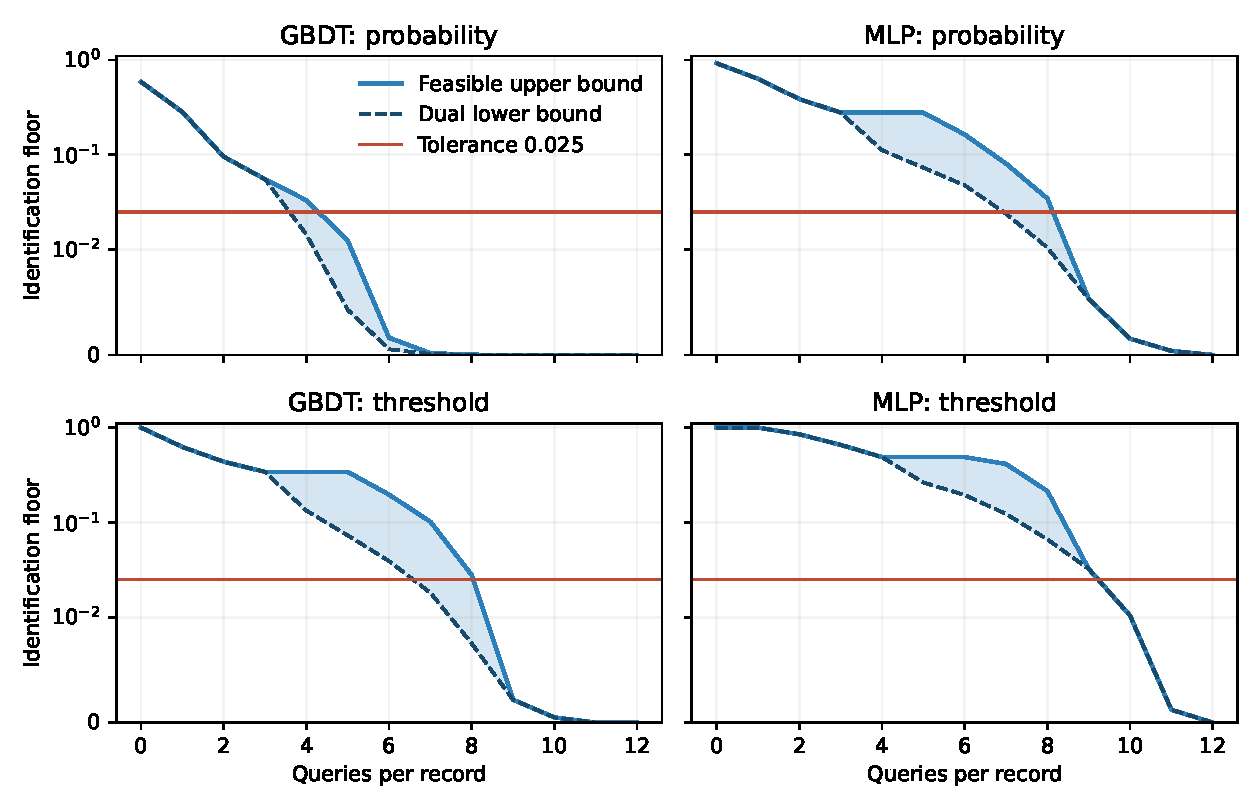
\includegraphics[width=.96\textwidth]{figures/budget_curves.pdf}
\caption{Median certified identification-floor brackets across five fixed WDBC splits. Solid curves are upper bounds, dashed curves lower bounds, and shading shows the remaining uncertainty. The horizontal line is the target 0.025. Upper and lower medians need not come from the same split. The vertical scale is linear below 0.01 and logarithmic above.}
\label{fig:budgetcurves}
\end{figure*}


\section{Analysis of a Genuine Planned-Missing Archive}\label{app:pisa}
\subsection{Observed forms, common target and acquisition constraint}
We use the national U.S. PISA 2012 student public-use file supplied by NCES
\citep{pisaus2014}. The OECD technical report, Chapter 3, describes random
allocation of three student questionnaires, with approximately equal
counts. Each has an eight-minute common part and two eleven-minute rotated
parts. The U.S. technical report describes the forms' A--B--C spiraling
and the required survey-weight analysis \citep{pisa2014,kastberg2014}.
Our analysis uses allocation probabilities $q_A=q_B=q_C=1/3$. The observed
form identifier is \texttt{QUESTID}; \texttt{FORMID} identifies a different,
computer-based assessment and must not be used for this purpose.

The nine predictors are the first three response items in each of
\texttt{ST29} (interest/motivation), \texttt{ST42} (anxiety/self-concept),
and \texttt{ST53} (learning strategies). Call these blocks $U,V,W$.
Forms A, B, C reveal $(U,W)$, $(U,V)$, $(V,W)$, respectively. The released
codes confirm that every selected item outside its assigned form has the
structural not-applicable code. Within a received form, ST29/ST42 responses
1 or 2 define endorsement; ST53 response 1 defines endorsement. All other
received responses, including item nonresponse or invalid codes, define
nonendorsement. Thus we estimate a contrast of recorded responses, not
the unobserved substantive answers of nonresponders. This convention does
not complete any structurally omitted block.

The common target \texttt{ST07Q01} asks about grade repetition in grades
1--6. Codes 2/3 define $Z=1$, and code 1 defines $Z=0$. We retain 4,752 of
4,978 records with a valid target report. The design-based interpretation
is conditional on this respondent population and assumes that common-part
response does not break the randomized allocation. A claim about all
students, including target nonresponders, would require further assumptions.
There are 1,582/1,590/1,580 retained records on A/B/C. No record has all
nine selected predictors. These are nine selected indicators within a
larger 30-minute questionnaire, not nine independent tests in the actual
survey protocol.

\subsection{Frozen ensembles trained from incomplete records}
We permute the 162 school IDs with seed 20261108. The first forty schools
train the old rule, the next forty train the new rule, and the remaining
82 form the audit domain. The corresponding valid-target record counts
are 1,115, 1,196 and 2,441. The audit contains 801/821/819 A/B/C forms.
School-level separation avoids training and evaluating on students in
the same school. Estimates and uncertainty below condition on the fitted
rules and the chosen audit domain; they do not include variation from
retraining the models.

For version $j\in\{0,1\}$, let
\[
 p_j(x)=\{f_{jU}(x_U)+f_{jV}(x_V)+f_{jW}(x_W)\}/3.
\]
Each component is a fifty-tree probability forest, trained only on records
receiving that block. Old/new component depths are two/three, respectively,
with minimum leaf size twenty, all three block features eligible at each
split, fixed independent seeds, and survey weights normalized to mean
one in fitting. Old block fits use 745/744/741 records; new fits use
805/786/801. There is no complete-record training or calibration sample.
The resulting contrast depends on all nine predictors. This is a
specified secondary model-comparison task, not a deployed educational
prediction system or a causal analysis of grade repetition.

\subsection{Why Brier comparison is identifiable on these actual forms}
For $K=3$ blocks, set
\[
 a_k=\frac{f_{0k}^2-f_{1k}^2}{9}
       +\frac{2Z}{3}(f_{1k}-f_{0k}),\qquad
 b_{k\ell}=\frac{2}{9}(f_{0k}f_{0\ell}-f_{1k}f_{1\ell}).
\]
Expanding the squared losses gives the pointwise identity
\[
 (p_0-Z)^2-(p_1-Z)^2=\sum_k a_k+\sum_{k<\ell}b_{k\ell}.
\]
Every single block is observed with probability $2/3$ and every pair with
probability $1/3$. On the form containing $k,\ell$, the score
$\tfrac32(a_k+a_\ell)+3b_{k\ell}$ is consequently unbiased. For randomized
accuracy the corresponding score is
$\tfrac{Y}{2}\{(f_{1k}-f_{0k})+(f_{1\ell}-f_{0\ell})\}$.
Both are evaluated entirely on received responses and the common label.

The same argument applies to an average of arbitrary block functions:
accuracy requires coverage of each block; Brier additionally requires
coverage of each interacting block pair. This is an application of the
observation-span criterion. A nonlinear transformation such as log loss
can involve three-block interactions that none of these forms observes.
The fact that every pair of blocks co-occurs does not identify arbitrary
functions of all three blocks.

For the optimized score, keep $q=1/3$ and solve the quadratic version of
\eqref{eq:fullprogram}. Each form has 64 binary cells; 169 distinct Fourier
terms occur across the three forms. The constraints are imposed separately
for the two labels. Estimate each form's joint cell--label frequencies
from the pooled old/new training schools, using survey weights within
that form and 0.1 uniform shrinkage. No assumption that these estimated
marginals form a compatible joint distribution is needed for unbiasedness.
The released tables satisfy the target identity on all 512 profiles and
both labels; the maximum numerical residual is $3.1\times10^{-16}$.

\subsection{Survey uncertainty and imputation comparator}
Let $w_i$ and $w_i^{(r)}$ be the supplied final and eighty replicate
weights. For frozen scores $H_i$, report the weighted mean
$\widehat\Delta=\sum_iw_iH_i/\sum_iw_i$ in the audit domain and
\[
 \widehat{\operatorname{se}}^2
 =\frac{1}{80(1-0.5)^2}
       \sum_{r=1}^{80}(\widehat\Delta^{(r)}-\widehat\Delta)^2.
\]
This is the documented Fay BRR calculation, not an iid Wald calculation.
The resulting normal intervals are survey-asymptotic intervals, not the
finite-sample minimax confidence guarantee. Conditional on sampled records
and their fixed weights, the weighted form-score mean is unbiased over
the stipulated form assignment; survey-population interpretation also
uses the survey's weighting and response assumptions.

We implement twenty independent chains of logistic multiple imputation
\citep{vanbuuren2011}, with fifteen sweeps per chain and fixed seeds. Only
the omitted block is imputed. Each conditional regression uses the other
eight predictors, observed target, reported sex, grade and log survey
weight. Coefficients use Laplace draws around a weakly regularized,
weighted logistic fit. This is a transparent working-model implementation,
not a claim to run the R \texttt{mice} package or an exact posterior sampler.
For each completed dataset we evaluate the frozen contrast and its Fay
variance. Rubin combination uses within-imputation mean variance
$\overline U$, between-imputation variance $B$, total
$\overline U+(1+1/20)B$, and the usual degrees-of-freedom adjustment.
These intervals depend on the imputation specification, its compatibility
with the target, and survey approximations; nominal coverage is not
verified without complete-data truth.

For randomized accuracy, optimized scores give 0.04142 with interval
$[0.03785,0.04500]$, block HT gives 0.04174 with
$[0.03814,0.04534]$, and logistic MI gives 0.04180 with
$[0.03825,0.04535]$. For Brier improvement, all intervals in
Table~\ref{tab:pisa} contain zero. Both probabilities stay below 0.5 on
the full cube (old range 0.112--0.231, new range 0.040--0.137), so
thresholded accuracy has identically zero contrast. The probability-loss
comparison is substantive only as a probability-quality target, not as
an improvement in these deterministic decisions. The agreement is useful evidence of
stability for this specified analysis, not evidence that the imputation
model is correct or that optimized scores dominate simpler scores.

Each predictor occurs on two forms, allowing nine marginal response
comparisons. On audit records, two unadjusted BRR comparisons have
$p<0.05$ (0.0479 and 0.0449); none meets $0.05/9$. The maximum estimated
difference is 0.0482. Random differences, form order, context and
nonresponse can all contribute. Failure to reject after correction does
not certify measurement invariance, and these marginal checks cannot
identify all unobserved joint response differences. No branching benefit,
MSE or coverage estimate is claimed from this archive.

\section{Independent Forest Updates and Binding Constraints}\label{app:forest}
\subsection{Complete prespecified grid}
The protocol fixes three datasets, twenty seeds 20261108--20261127,
four nested feature counts $m\in\{3,6,9,12\}$ and cap three. WDBC uses
100 old-training, 200 new-training and 269 evaluation records; Spambase
uses 500, 1,000 and 3,101; Ionosphere uses 60, 120 and 171. We binarize
strictly above pooled training medians. Among columns varying on these
training records, take twelve evenly spaced column indices, then the
first $m$. Feature selection does not inspect labels. Each version fits
twenty depth-three trees with bootstrap samples, square-root feature
sampling and minimum leaf size $\max(3,n_{\rm old}/30)$ rounded down.
The versions have separate training records and seeds. The target is
$Y(p_1-p_0)$ for probability averages; thresholding a forest may destroy
degree-three identification.

Training records also fit the reference marginals, with uniform shrinkage
0.1 and a design floor $q_\iota\ge0.05/|\A|$. These are records used to fit
the evaluated models, so their in-sample paired loss is not an independent
target audit. No fresh complete calibration sample is excluded from the
acquisition accounting. Exact variances below condition on the fitted
models, reference and empirical held-out law. Repeated splits reuse
records, and their quantiles describe the experiment rather than
independent population replications.

\begin{figure}[ht]
\centering
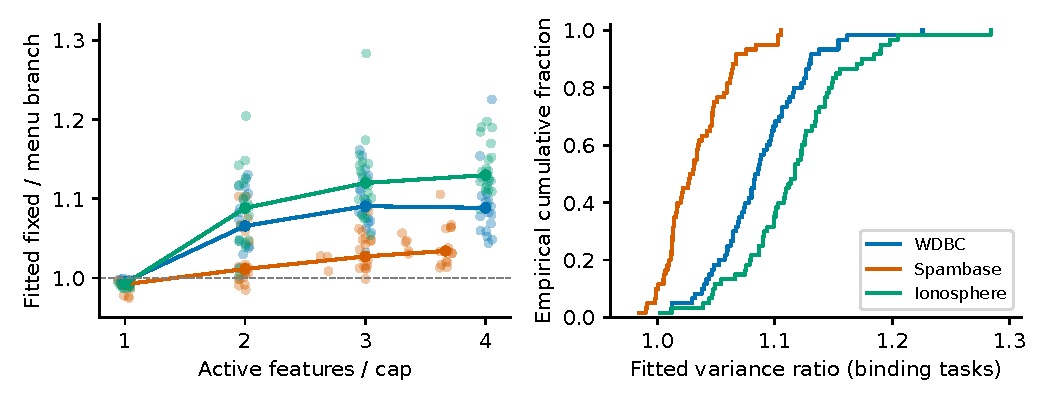
\includegraphics[width=.95\textwidth]{figures/forest_binding.pdf}
\caption{Every forest comparison and the distribution of the 180 binding
cases. Lines in the left panel join dataset medians across candidate
feature counts; models are refitted at each count, so the plot is not a
causal or monotonicity claim about active features. The right panel shows
the full empirical distribution.}
\label{fig:forestbinding}
\end{figure}

\subsection{Branching denominator and numerical bounds}
The fixed menu contains every size-three coordinate set. The tested
branch menu contains those forms and all forty component trees of the two
forests. Joint optimization uses the observed leaf, label and selected
tree, with the same pointwise target identity as fixed-form optimization.
It does not read all forest predictions on one person. We also implement
a centered random-component score: for signed forest weights $w_j$,
reference centers $\mu_j$, and $c=\sum_jw_j\mu_j$, return
\[
 H=Y\left(c+\frac{w_J\{f_J(X)-\mu_J\}}{q_J}\right).
\]
Reference residual second moments choose $q_J$, with the same 0.05 uniform
floor. The selected component's depth is at most three.

For each menu the reference-fitted procedure is evaluated on the held-out
law. Its ratio can be below one: fitting error and the menu-specific
positive probability floors can make the larger menu's implemented score
worse. This is not a reversal of the optimal information comparison.
Separate population-oracle programs omit the floor and jointly optimize
the design and all cell scores. Their primal values and dual witnesses
give numerical intervals, with explicit zero-mass-cell projections and
full-cube unbiasedness repair. These are floating-point checks, not exact
rational certificates. The maximum oracle ratio interval width is 0.00749;
the maximum score or zero-cell residual is $2.3\times10^{-15}$.

Let $W_F$ denote the unrestricted fixed-form optimum and $W_M$ the optimum
of the supplied branch menu. Since the menu is feasible,
$W_{\rm branch}\le W_M$, so $W_F^L/W_M^U$ lower-bounds
$W_F/W_{\rm branch}$. In contrast $W_F^U/W_M^L$ is only an upper endpoint
for $W_F/W_M$. The full-information variance supplies a separate, typically
looser upper bound $W_F^U/\Var(Yd)$ for the unrestricted ratio. We do not
infer that every depth-three adaptive strategy is close to the fixed
optimum. None of the tested fitted ratios exceeds 1.5; their maximum is
1.284. The largest oracle-menu lower endpoint is 1.207.
Appendix~\ref{app:forestexact} computes $W_{\rm branch}$ over all
depth-three trees by certified column generation, on a full-support version
of the held-out law. The exact ratios have median 1.51 on the binding tasks,
so this supplied menu understates the intrinsic ratio substantially.

\begin{table}[ht]
\centering
\caption{Full independent-forest grid: each row contains 20 fixed splits. Fitted ratio quantiles describe variation across overlapping splits; they are not confidence intervals. Oracle intervals concern the specified branch menu.}
\label{tab:forestdetail}
\small
\begin{tabular}{llrrrrr}
\toprule
Data & $m$ & Active median & Fitted median & Fitted 10--90\% & Oracle lower & Oracle upper \\
\midrule
Ionosphere & 3 & 3 & 0.992 & [0.987, 0.995] & 1.0000 & 1.0000 \\
Ionosphere & 6 & 6 & 1.088 & [1.036, 1.143] & 1.0699 & 1.0707 \\
Ionosphere & 9 & 9 & 1.120 & [1.076, 1.158] & 1.0992 & 1.0994 \\
Ionosphere & 12 & 12 & 1.130 & [1.107, 1.190] & 1.1053 & 1.1058 \\
Spambase & 3 & 3 & 0.992 & [0.978, 0.995] & 1.0000 & 1.0000 \\
Spambase & 6 & 6 & 1.011 & [0.991, 1.078] & 1.0258 & 1.0258 \\
Spambase & 9 & 9 & 1.027 & [1.011, 1.059] & 1.0332 & 1.0335 \\
Spambase & 12 & 11 & 1.034 & [1.016, 1.064] & 1.0362 & 1.0364 \\
WDBC & 3 & 3 & 0.995 & [0.991, 0.998] & 1.0000 & 1.0000 \\
WDBC & 6 & 6 & 1.066 & [1.012, 1.117] & 1.0861 & 1.0878 \\
WDBC & 9 & 9 & 1.091 & [1.062, 1.139] & 1.0941 & 1.0976 \\
WDBC & 12 & 12 & 1.089 & [1.052, 1.133] & 1.0810 & 1.0845 \\
\bottomrule
\end{tabular}
\end{table}


\subsection{Structural ties in the independent-tree benchmark}\label{app:binding}
The eight-feature experiment in Appendix~\ref{app:medium} must be stratified
per task, rather than comparing separate medians of active feature count
and cap. Among probability-output contrasts, 39/45 SUSHI and 21/25 SAPA
tasks are binding. Within those strata, median population ratios are
1.353 and 1.295; median global ratios remain 1.000. The other ten tasks
have a form that computes their contrast exactly. Among 58 nonzero
thresholded contrasts, 35/39 SUSHI and 17/19 SAPA tasks are nonbinding.
The six binding threshold tasks have median population ratios 1.289 and
1.360 in the two datasets. Thus nonbinding budgets explain most
thresholded ties, not the probability-output results. The released
\texttt{independent\_binding\_strata.csv} contains every stratum.

\section{Cost Regimes Under a Relaxable Cap}\label{app:costchoice}
\begin{figure}[ht]
\centering
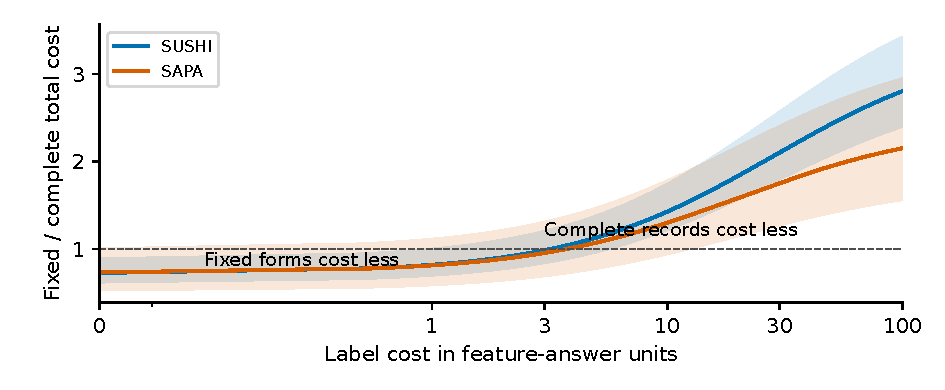
\includegraphics[width=.85\textwidth]{figures/cost_choice.pdf}
\caption{Fixed-form versus complete-record cost on all 70 controlled tree
tasks, allowing complete acquisition. Lines are medians, bands are the
10th--90th percentiles. Planning targets half-width 0.025, includes integer
sample counts and a minimum of thirty, and conditions on the reference.
Under an immutable cap, the complete-record alternative is unavailable.
When branching can compute the target and is permitted, its lower feature
count and full-information variance make it the natural comparator.}
\label{fig:costchoice}
\end{figure}
At zero label cost the median planned fixed/complete ratios are 0.726 on
SUSHI and 0.731 on SAPA; at label cost ten they are 1.427 and 1.299.
These conditional cost curves do not price an independent complete
reference as free: same-population reference records should first be used
as audit observations. Transferred or restricted calibration requires its
own analysis. An uncorrected imputation method cannot be assigned a
universal winning region using label cost alone, because its bias,
sample size and desired inference guarantee also matter.


\section{Reproducibility and Research Methods}
The anonymous supplement contains code, numerical certificates, aggregate
results, simulation standard errors, and figure/table generators. Source data
are obtained separately with pinned checksums. The SUSHI loader also verifies
a normalized profile fingerprint because the creator's legacy archive and
current PrefLib profile differ. Individual SUSHI rankings may not be
redistributed; no individual survey records are supplied.

Checks cover 21,276 exact rational hybrid-budget inequalities, six independent
small conic programs, binary and ordinal profile-cell formulations, and five
full-support local-efficiency comparisons. EM is checked against direct
maximization of its penalized likelihood. Release checks verify task counts,
comparator populations, primal/dual bounds, pilot-risk accounting, and
interval simulation errors. Symbolic and numerical checks are also supplied.

These finite checks support the implementations and written derivations;
they do not replace proofs of general statements. The product counterexample
has a separately released rational certificate checked exactly on all 256
profiles. The unrestricted-menu experiment enumerates every eligible form
on all 70 binary tasks and releases its population witnesses. Nonlinear-model
floor certificates use exact integer nullspace checks and rational endpoint
evaluation on the released prediction grids. The one-sided address formula
has an analytic proof and exact small-instance primal/dual checks.
All 1,048 retained release checks and 50 new archive/forest checks pass.
The new checks verify actual-form observability, the Brier block
decomposition, MI summary arithmetic and the complete forest grid,
including a separate address instance with known optima. The proper-loss extension is
checked on every profile and both labels of
an independent toy cube. The budget-curve release contains all 260
recorded cap/contrast cases, with separately implemented Python-integer
Walsh and rational endpoint checks; age-transfer summaries retain every
nonzero case and explicitly record zero contrasts.
A generative language
model participated in formulating research questions, deriving and checking
proof arguments, implementing analyses, and drafting the manuscript.
